\chapter{Designing and Fabricating the Enclosure: 3D Modeling and Printing}
\label{cap:3dModelingAndPrinting}


Designing and fabricating enclosures for electronic devices involves choosing the most suitable 
fabrication method. Various methods exist, ranging from traditional machining and molding 
techniques to more modern additive manufacturing processes. Among these, 3D printing has become 
one of the most accessible and cost-effective methods, especially for small-scale productions and 
prototypes.

Unlike traditional manufacturing processes that may require expensive tooling and setups, 3D 
printing has minimal upfront costs to get started. This makes it particularly attractive for rapid 
prototyping and custom design iterations. The ability to create complex geometries and designs 
with relative ease also contributes to its popularity in the field of electronics.

In this chapter, the process of designing and fabricating the enclosure for the employee time 
tracking device using 3D modeling and printing techniques is explored. The chapter discusses the 
design considerations, the software tools used for modeling, and the intricacies of the 3D 
printing process. Additionally, it examines the challenges encountered and the solutions 
implemented during this phase.


%
%   3D MODELING
%

\section{3D Modeling}

3D modeling plays a crucial role in the design and fabrication of the enclosure for the employee 
time tracking device. It enables precise visualization and customization of the physical form of 
the device, accommodating its electronic components and ensuring functional and aesthetic 
requirements are met. This section explores the process of 3D modeling, detailing the software 
tools utilized, the design considerations, and the iterative development of the enclosure design. 

\subsection{An Iterative Process}

The first step in designing the enclosure was to decide on a general shape. The primary objective 
was to create an enclosure that was as compact as possible while remaining visually appealing and 
functional. A rectangular shape was chosen, with the layout designed to maximize usability and 
accessibility. The top third of the enclosure would be occupied by the screen, providing a clear 
display for users, while the lower two-thirds would house the NFC reader, the Raspberry Pi, and 
the PCB. This can be seen in Figure \ref{fig:enclosure_front}.

\begin{figure}[h]
	\centering
	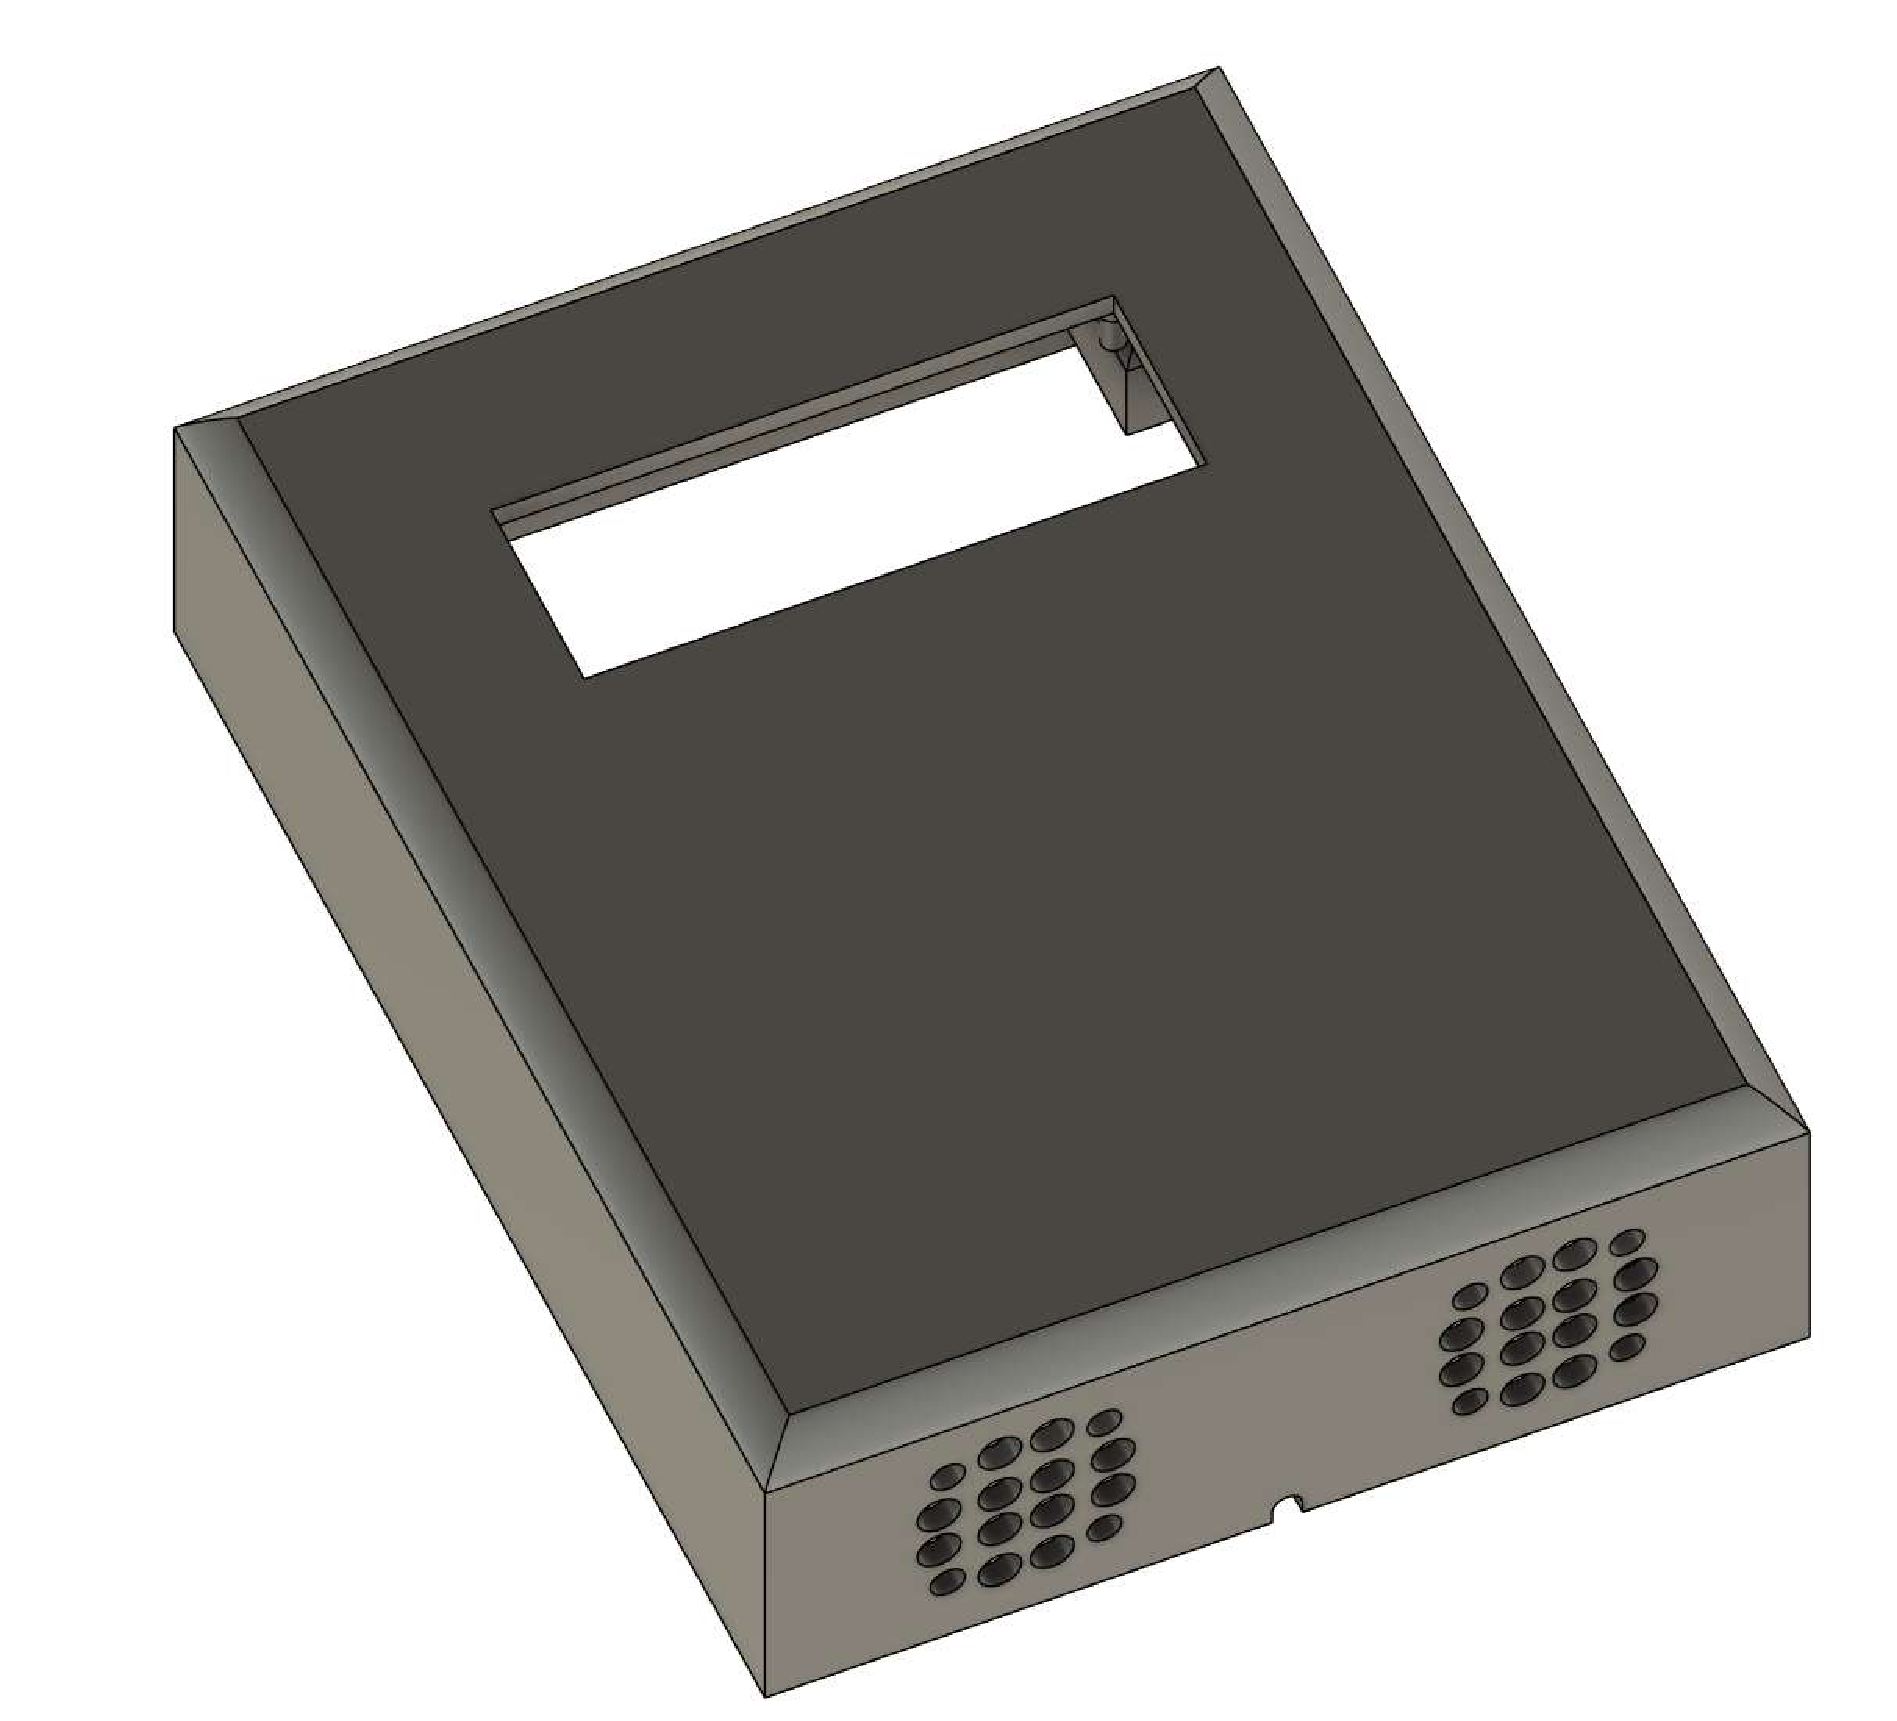
\includegraphics[width = .5\textwidth]{Imagenes/Vectorial/enclosure_front.pdf}
	\caption{Enclosure view from the top}
	\label{fig:enclosure_front}
\end{figure}

To bring this design to life, Fusion 360\footnote{Fusion 360's Website: 
\url{https://www.autodesk.es/products/fusion-360/overview}}, developed by Autodesk, was selected 
as the modeling software. Fusion 360 is an industry-leading solution renowned for its versatility 
and widespread use in 3D modeling for various applications, including product design and 
engineering.

Ensuring the secure attachment of the components to the enclosure was critical. The mounting holes 
present in the NFC reader's board, the display, and the PCB were utilized for this purpose. 
Precise measurements were taken using a caliper to model the studs accurately in Fusion 360. These 
measurements ensured that the components would fit snugly and securely within the enclosure.
Considering that the device had to be as compact as possible, the NFC reader and the PCB were 
stacked one on top of the other, making for an extremely compact design.

In the first design iteration, threaded studs were incorporated into the model. Corresponding nuts 
were also designed to secure these studs. Although the threads functioned as intended, they proved 
to be problematic. The studs, being less than 3 millimeters in diameter, were too fragile. They 
tended to break easily if the enclosure was dropped, and the threads often sheared off, making it 
difficult to release the components without breaking the studs. This initial challenge highlighted 
the need for a more robust solution in subsequent design iterations.

It is also worth noting that even with the studs at the full 3-millimeter diameter, they remained 
fragile and prone to breaking when dropped. This issue manifested during testing, necessitating a 
more robust solution.

Consequently, walls were added to surround the NFC board and the PCB. These walls featured extra 
support on their lower half but lacked support near the top. This design allowed the walls to 
act like springs during a drop, absorbing impacts and preventing the boards from breaking the 
studs. This solution proved highly effective and was incorporated into the final design. This 
can be seen in Figure \ref{fig:enclosure_walls}.

\begin{figure}[h]
	\centering
	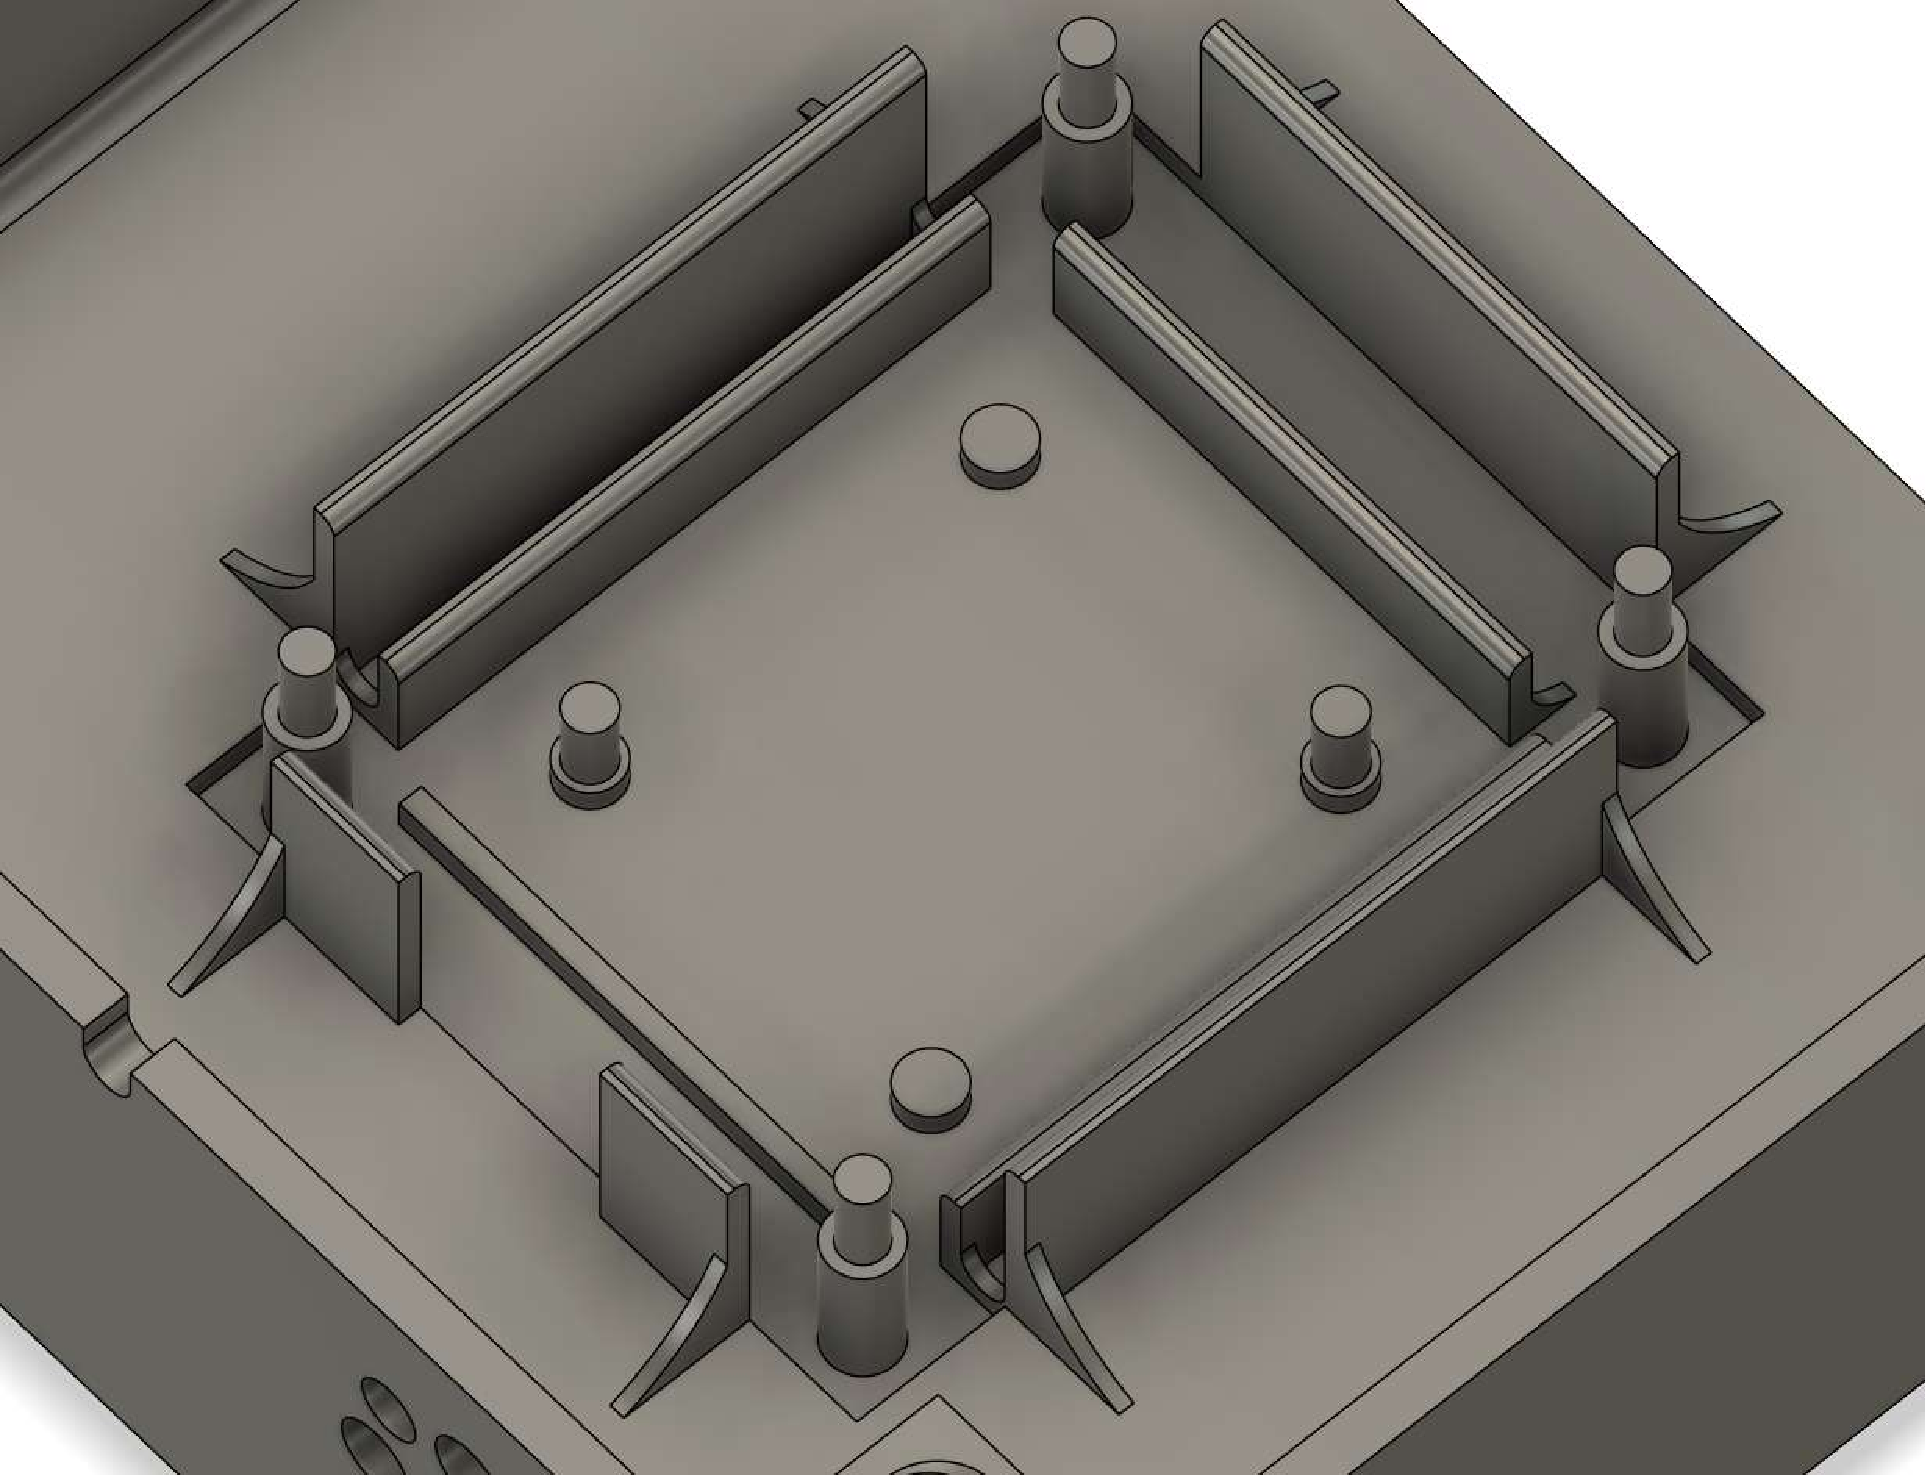
\includegraphics[width = .5\textwidth]{Imagenes/Vectorial/enclosure_walls.pdf}
	\caption{Enclosure's ``walls''}
	\label{fig:enclosure_walls}
\end{figure}

However, a new issue arose with the removal of the threaded studs: there was no way to prevent the 
components from moving up and down or shooting out of their positions. The solution came in the 
form of a backplate that would be screwed on the back of the enclosure. The height of the 
device was designed so that the backplate would press the Raspberry Pi Pico against the PCB and 
the base of the studs, preventing any movement. For the LCD display, four hollow cylinders were 
designed to press against the back of the LCD, ensuring it remained securely in place. This can be 
seen in Figure \ref{fig:backplate_front}. Notably, the LCD display did not require additional 
walls for support, as it was already held in place by protruding outside the enclosure. In this 
way, the final design successfully addressed the issues of component stability and impact 
resistance, ensuring a robust and reliable enclosure for the device.

\begin{figure}[h]
    \centering
    \begin{minipage}[b]{0.49\textwidth}
        \centering
        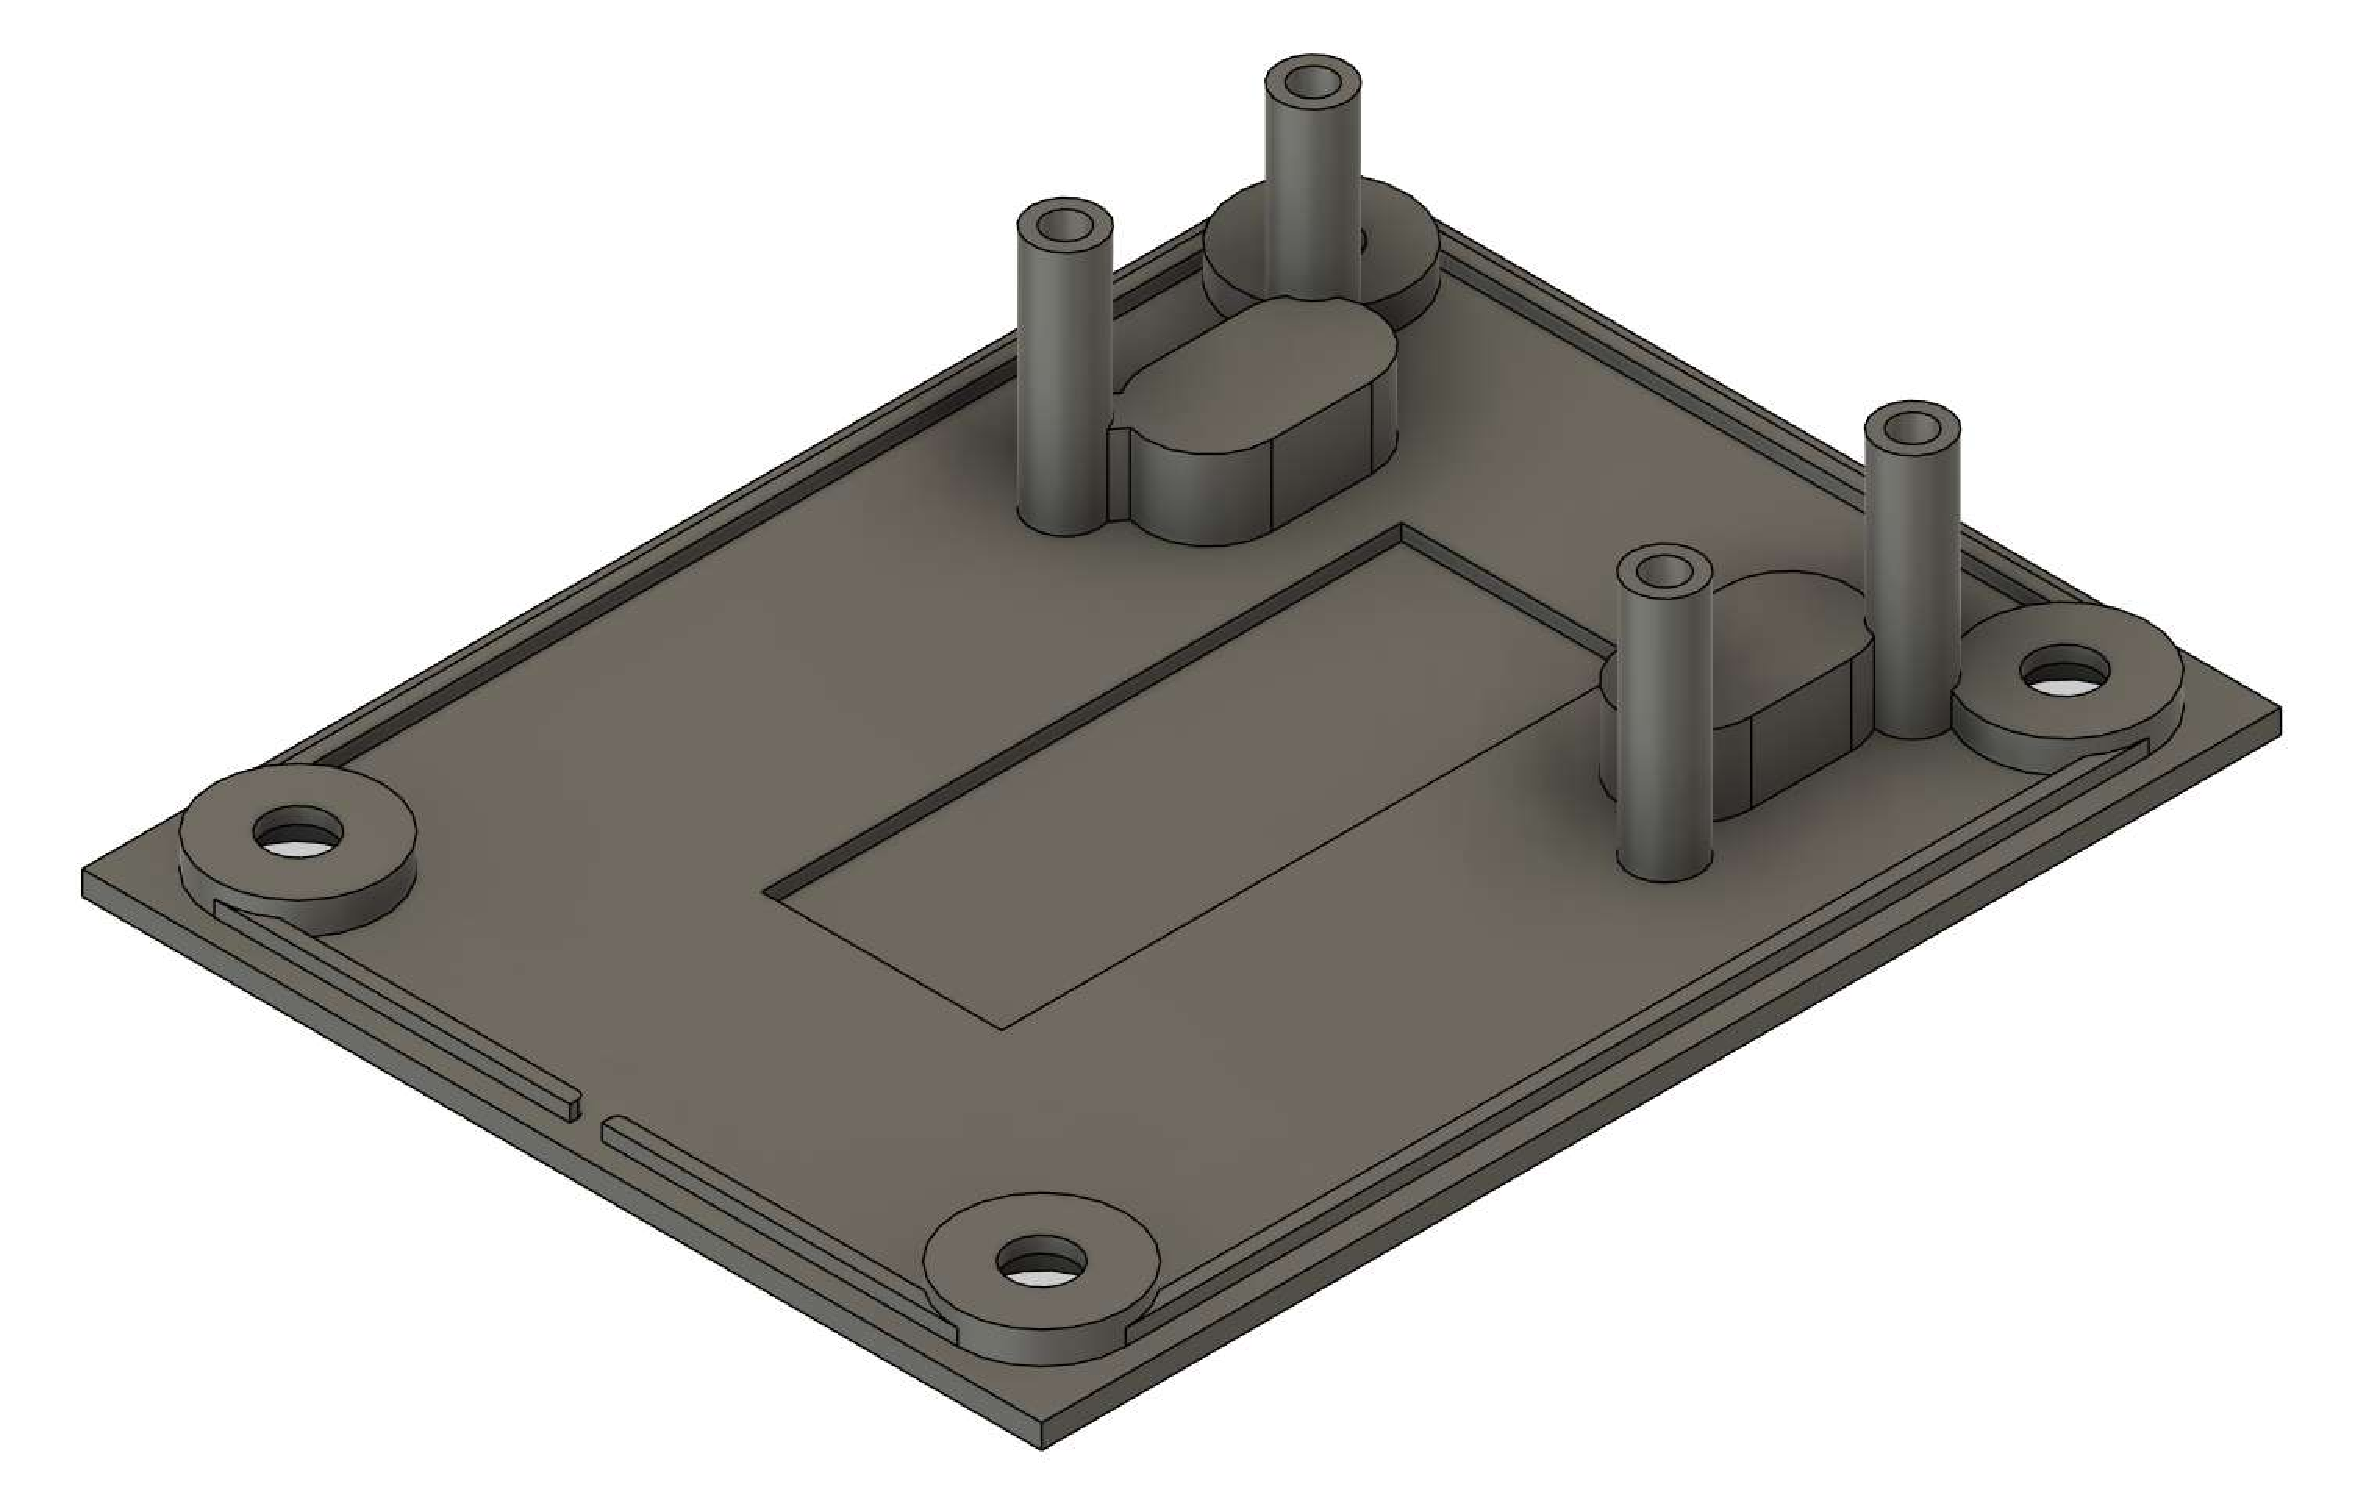
\includegraphics[width=1\textwidth]{Imagenes/Vectorial/backplate_front.pdf}
        \caption{Front side of the enclosure's backplate}
        \label{fig:backplate_front}
    \end{minipage}
    \hfill
    \begin{minipage}[b]{0.49\textwidth}
        \centering
        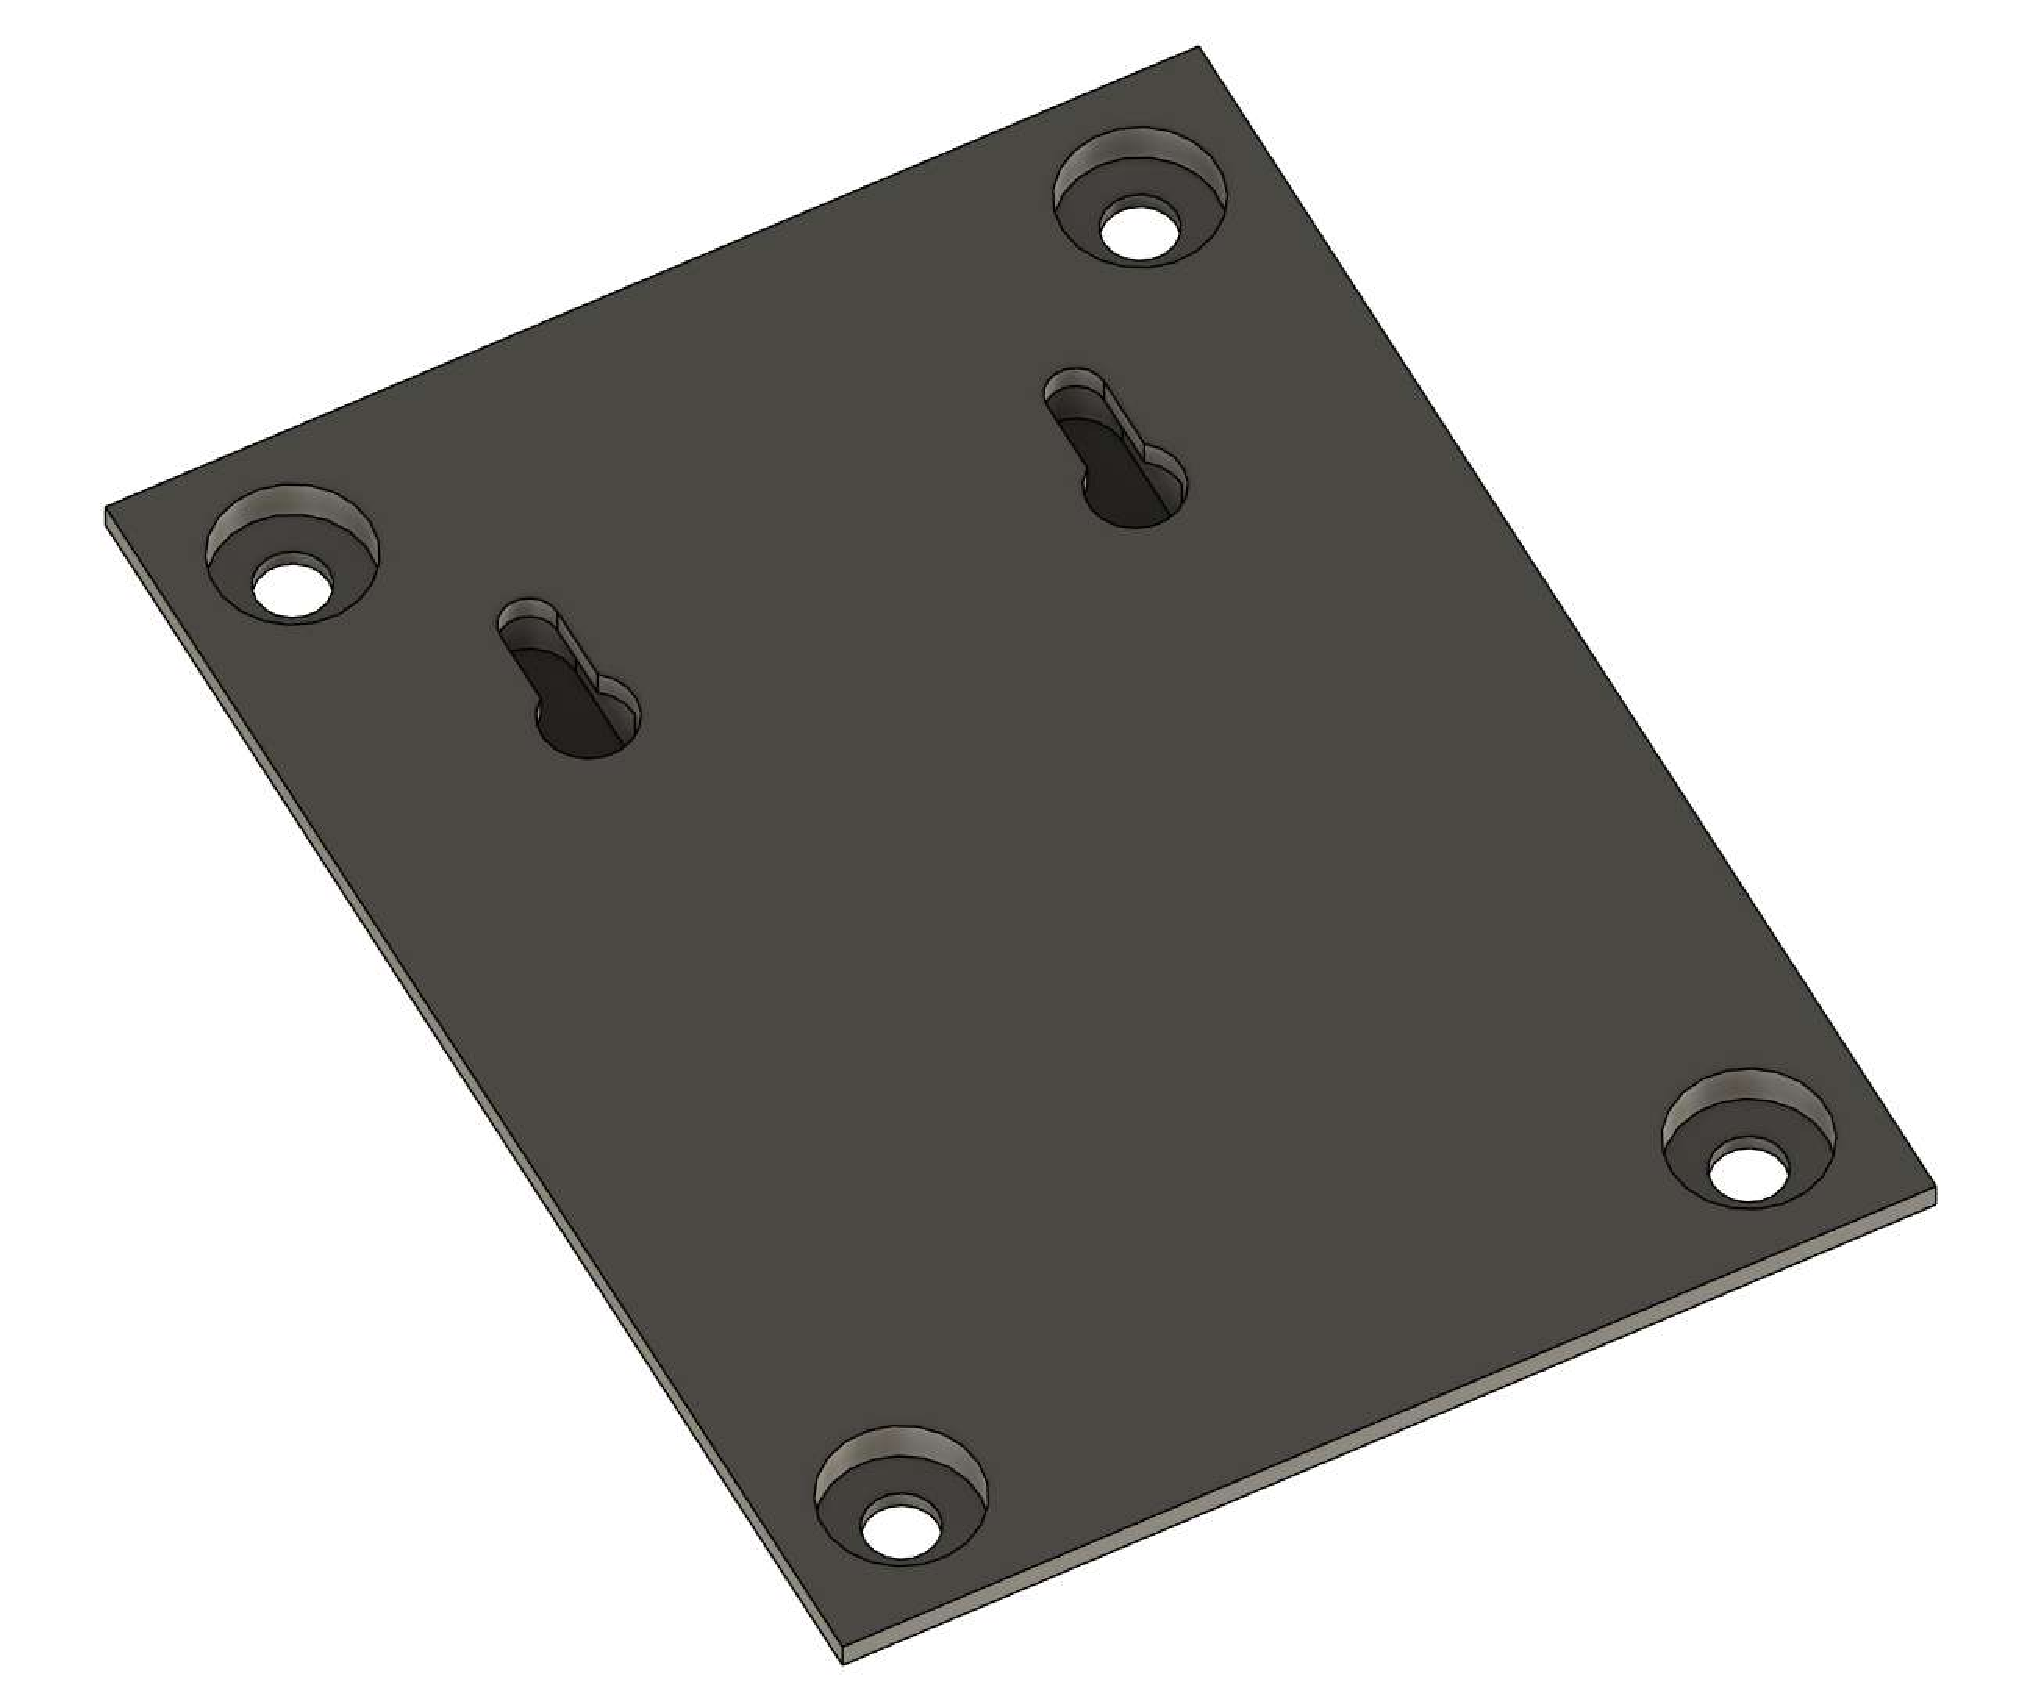
\includegraphics[width=1\textwidth]{Imagenes/Vectorial/backplate_back.pdf}
        \caption{Rear side of the enclosure's backplate}
        \label{fig:backplate_back}
    \end{minipage}
\end{figure}

Another challenging aspect of the design was the mounting mechanism for attaching the backplate to 
the enclosure. Ultimately, it was decided that both parts would be secured together using screws, 
which would be modeled and 3D printed for simplicity. This design required incorporating a 
threaded section on the enclosure side to tighten the screws.

Additionally, there is a recess surrounding the screw holes on the backplate. This recess 
accommodates the screw heads, ensuring they fit flush within the backplate and do not protrude, 
which allows for flat mounting to a wall.

Another important feature of the backplate is the perimeter that protrudes along its edge, as can 
be seen in Figure \ref{fig:backplate_front}. This perimeter holds the backplate laterally, so the 
screws only need to keep the backplate and the enclosure together, without bearing any lateral 
forces. This design detail enhances the structural integrity and durability of the assembled 
enclosure. Moreover, mounting holes were added, for the device to be wall-mounted. This detail can 
be seen in Figure \ref{fig:backplate_back}.

\begin{figure}[h]
	\centering
	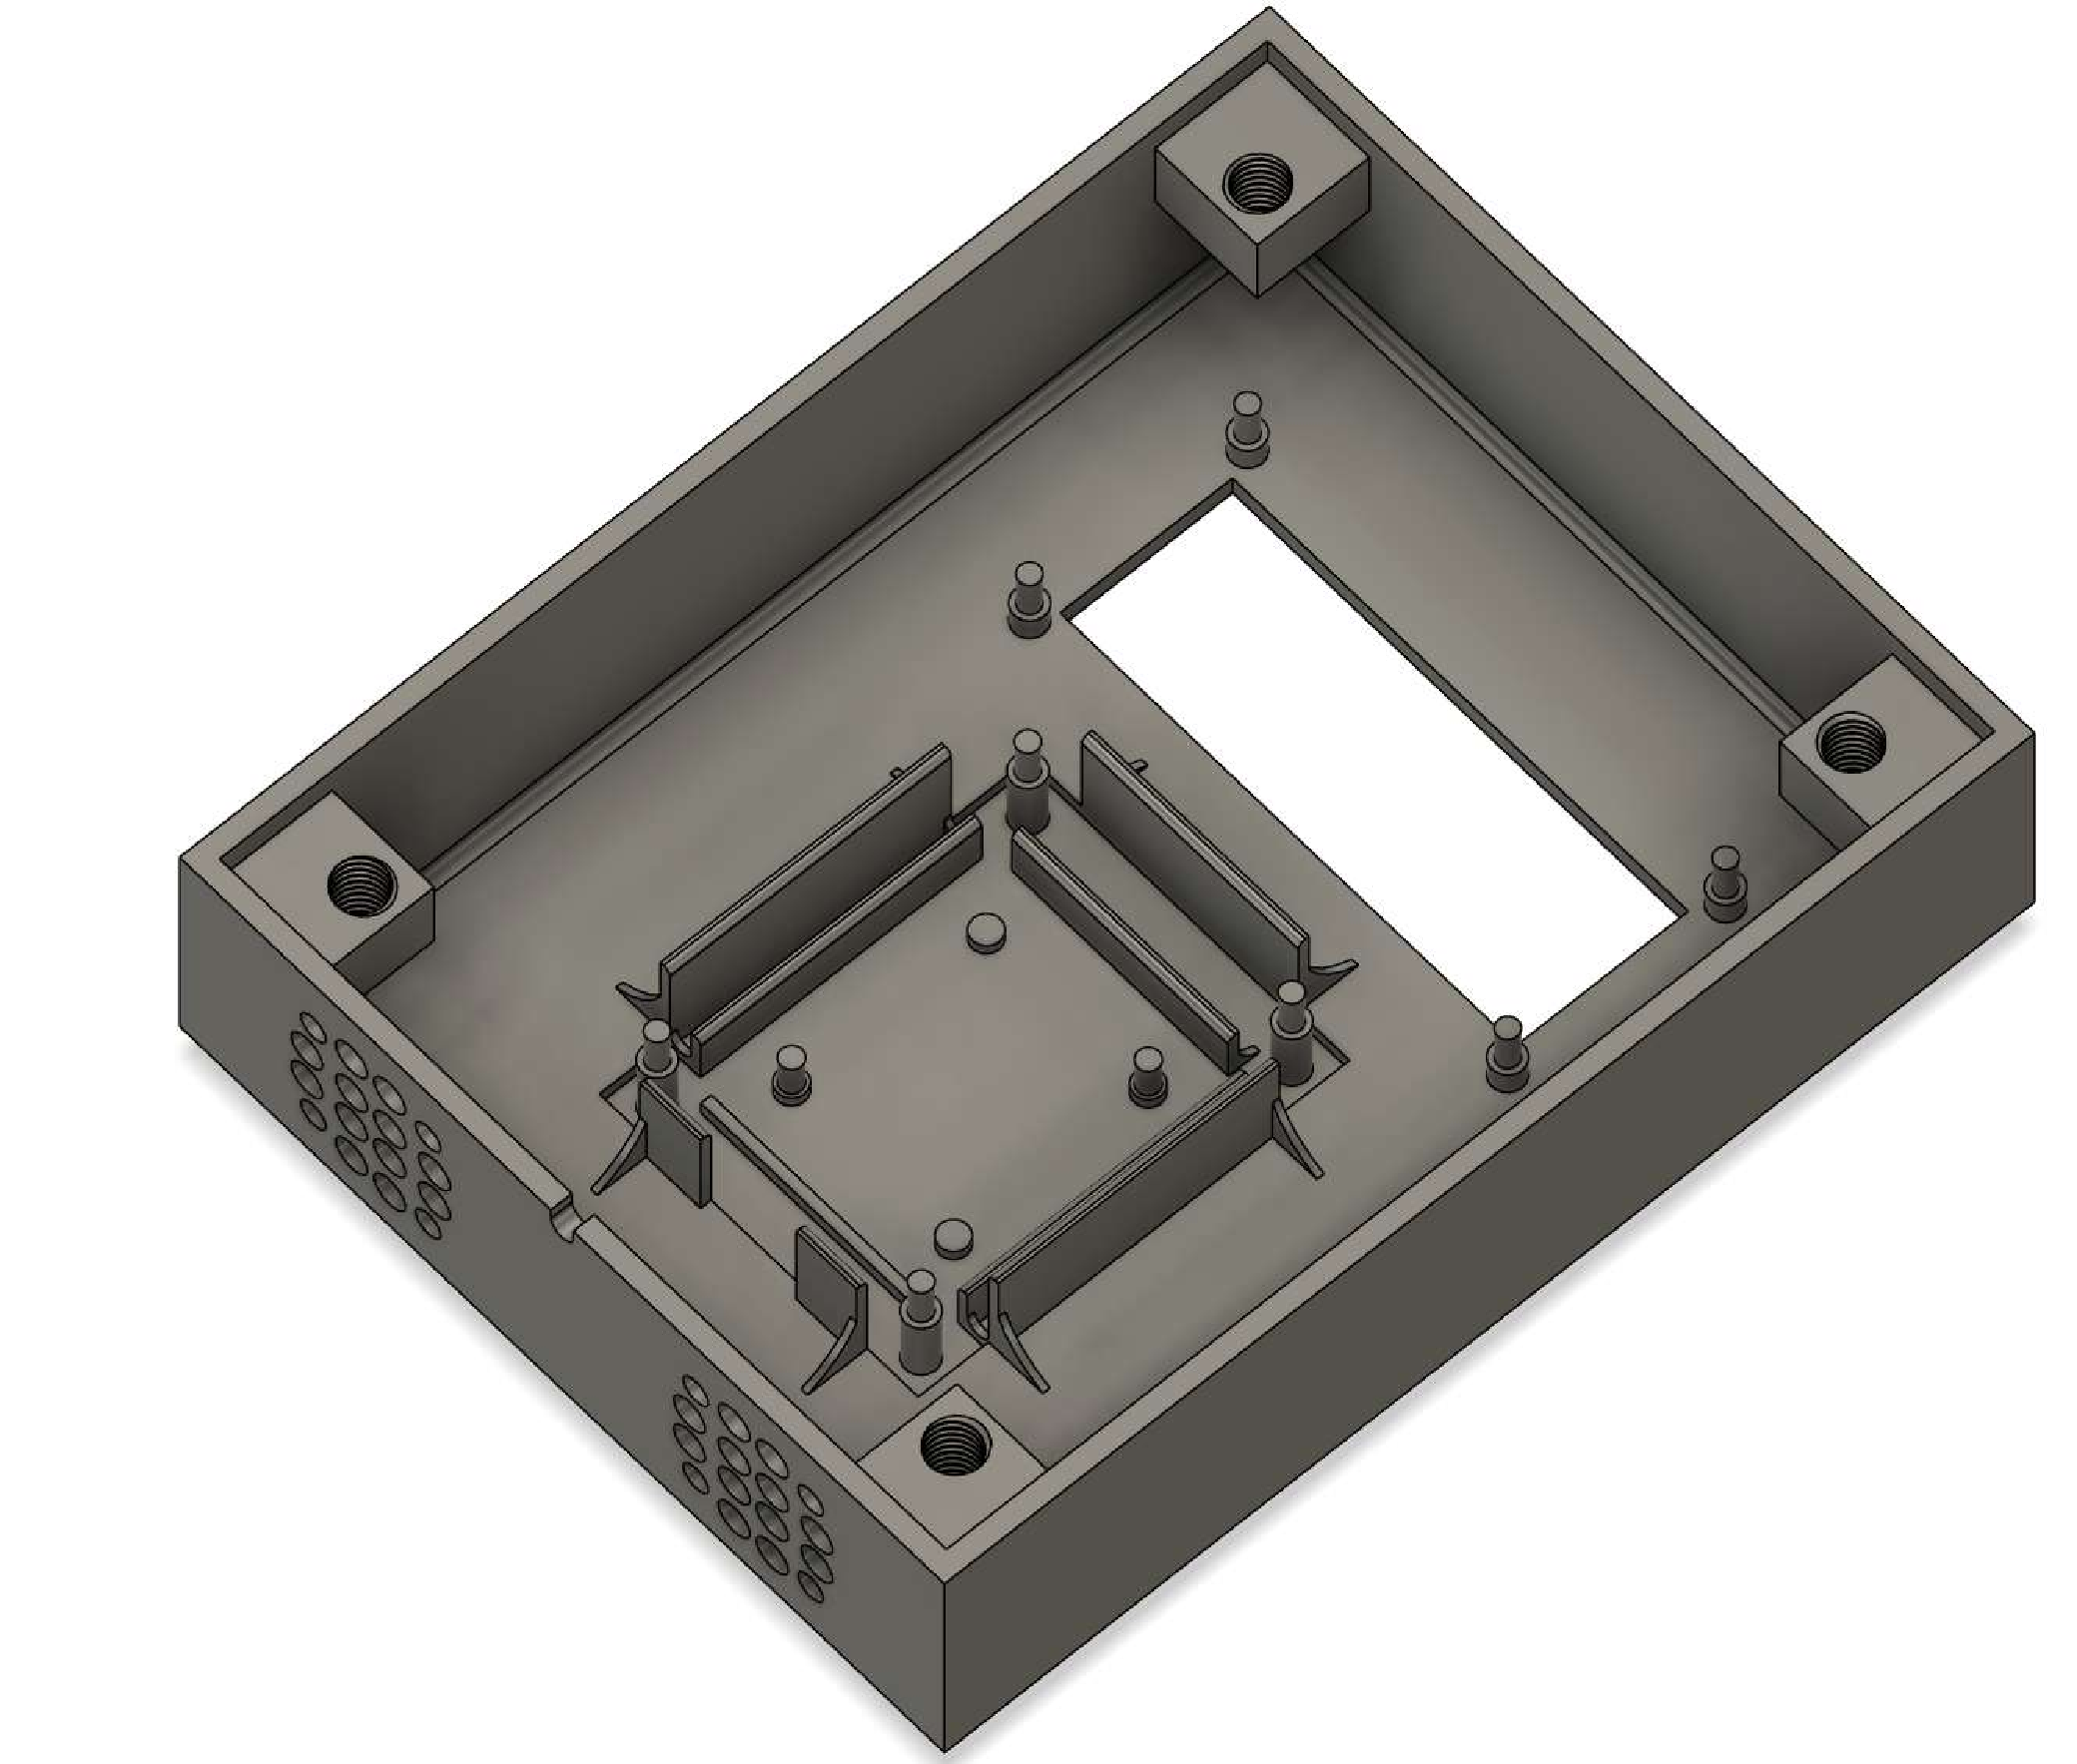
\includegraphics[width = .5\textwidth]{Imagenes/Vectorial/enclosure_back.pdf}
	\caption{Enclosure view from the back}
	\label{fig:enclosure_back}
\end{figure}

Details have already been provided regarding the mounting mechanism for the backplate to the enclosure. Now, the modifications on the enclosure-side will be explored.

A separate component was designed specifically to contain the threads that the screws 
would screw into. These threaded components were then placed in all four corners of the enclosure, 
positioned at the correct distance from the top to ensure the backplate fits flush against them. 
The individual threaded component is illustrated in Figure \ref{fig:enclosure_mounting}, while all 
four components integrated into the enclosure are shown in Figure \ref{fig:enclosure_back}.

\begin{figure}[h]
    \centering
    \begin{minipage}[b]{0.49\textwidth}
        \centering
        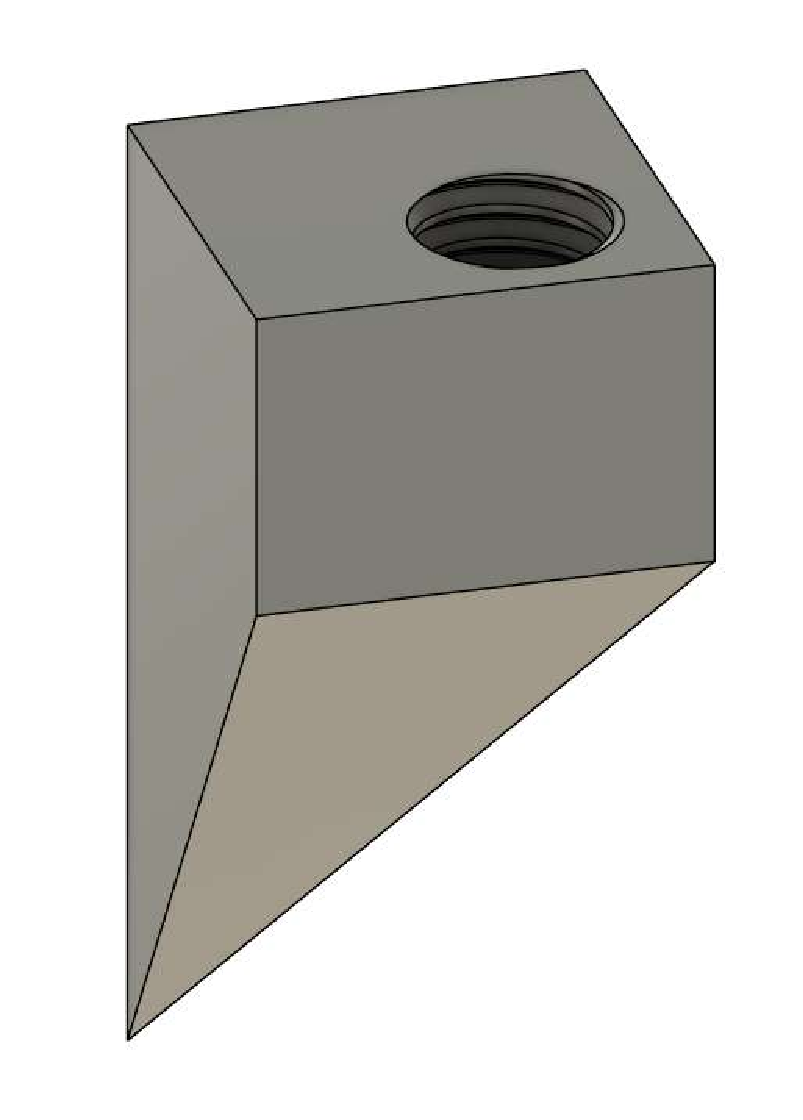
\includegraphics[width=.7\textwidth]{Imagenes/Vectorial/enclosure_mounting.pdf}
        \caption{Enclosure's mounting component}
        \label{fig:enclosure_mounting}
    \end{minipage}
    \hfill
    \begin{minipage}[b]{0.49\textwidth}
        \centering
        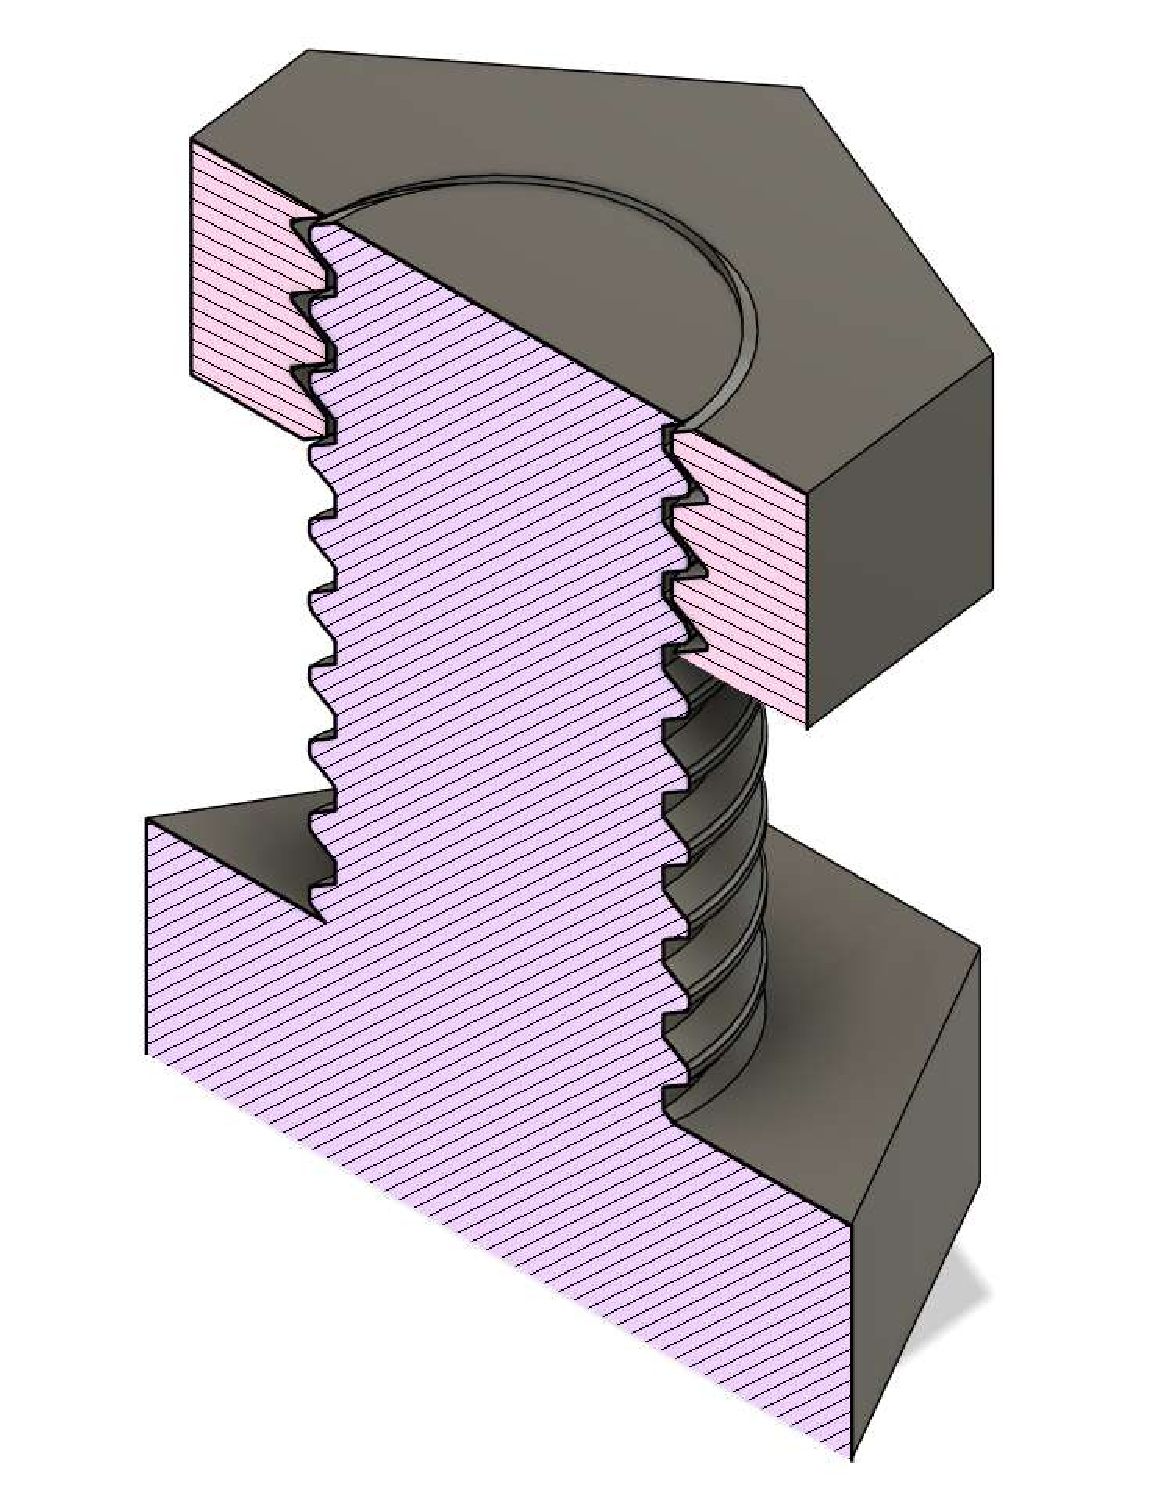
\includegraphics[width=.7\textwidth]{Imagenes/Vectorial/screw_cross_section.pdf}
        \caption{Screw's cross section}
        \label{fig:screw_cross_section}
    \end{minipage}
\end{figure}

Additionally, the screws were 3D printed and modeled using the threading tool in Fusion 360. This 
tool facilitated the creation of an M8 threaded screw, with a diameter of 8 millimeters. To ensure 
functionality, the screw was tested with a nut to verify that it could be smoothly screwed in and 
reused. The cross-section of the screw and nut assembly is illustrated in Figure 
\ref{fig:screw_cross_section}.

The final design details include ventilation holes at the bottom of the enclosure and a slot for 
cable routing. The ventilation holes are intended to allow air circulation, particularly if the 
enclosure is exposed to direct sunlight, to prevent heat buildup. The slot provides a pathway for 
the power cable. Both features are illustrated in Figure \ref{fig:enclosure_back}.


%
%   3D PRINTING
%

\section{3D Printing}

After completing the design of the enclosure, the next crucial step is to bring the digital model 
into the physical world through 3D printing. It is important to note that 3D modeling and printing 
were not strictly sequential processes but rather iterative and concurrent. This allowed for rapid 
prototyping and real-time adjustments to the design based on the physical prototypes. In this 
section, the focus will be on the 3D printing process itself, including the selection of 
materials, the configuration of the printer, and the iterative testing required to achieve a 
functional and durable final product. The flexibility and precision of 3D printing make it an 
ideal method for fabricating custom enclosures for electronic devices, enabling quick refinements 
and improvements throughout the development process.

There are two primary types of 3D printing technologies: \textit{Fused Deposition Modeling} (FDM) 
and \textit{Stereolithography} (SLA). FDM printers work by melting and extruding thermoplastic 
filament through a heated nozzle, which deposits the material layer by layer to build up the 
object. This method is known for its affordability, ease of use, and the ability to produce 
durable parts, making it ideal for creating functional prototypes and larger objects. However, FDM 
prints may have visible layer lines and may require post-processing for a smoother finish.

On the other hand, SLA printers use a laser or projector to cure liquid resin layer by layer. The 
resin hardens upon exposure to light, resulting in highly detailed and smooth parts. While SLA 
printing is excellent for intricate designs and small parts due to its high resolution, it can be 
more expensive because of the cost of resin and the need for post-processing. Additionally, the 
build volume of SLA printers is typically smaller compared to FDM printers \cite{fdm_vs_sla}.

For this project, FDM printing is the better choice. It is more cost-effective, with both printers 
and filament materials being more affordable. The thermoplastic materials used in FDM printing are 
durable and suitable for functional parts that need to withstand handling and usage. Furthermore, 
FDM printers are easier to set up and operate, which is beneficial for in-house production. They 
also offer larger build volumes, allowing for the printing of larger enclosures in a single piece, 
reducing the need for assembly. Overall, FDM printing provides a practical balance of cost, 
durability, and ease of use, making it well-suited for producing the enclosures needed for this 
project.

\subsection{Choosing a 3D Printer}

Given that the production of the enclosures would be done in-house, it was necessary to purchase a 
3D printer. The market for 3D printers spans a wide range of price points, from approximately 200€ 
to several thousand euros.

For the sake of simplicity, 3D printers can be categorized into three general types based on their 
price points: budget (200€ to 600€), mid-range (600€ to 1500€), and high-end (1500€ and above). 
While this is a broad approximation and may not apply to all printers (and in fact, it does not 
even properly cover industrial 3D printers, which may be well above 10.000€), it serves as a 
useful framework for understanding the options available on the market for this project.

The following information is based on merging many sources and adapting them to this project 
\cite{3dprinter_cost_1} \cite{3dprinter_cost_2} \cite{3dprinter_cost_3}. 

\subsubsection*{3D Printers in the Range of 200 to 600 Euros}

\begin{itemize}
    \item \textbf{Capabilities}: Printers in this price range are typically entry-level models 
    suitable for beginners and hobbyists. They offer basic functionalities for printing small to 
    medium-sized objects with decent accuracy.
    \item \textbf{Features}: These printers usually have a single extruder and a limited build 
    volume. They may lack advanced features such as automatic bed leveling, filament sensors, and 
    Wi-Fi connectivity.
    \item \textbf{Limitations}: While affordable, printers in this range may have lower build 
    quality, resulting in less reliable prints. They may require more manual calibration and 
    maintenance compared to higher-end models.
\end{itemize}

\subsubsection*{3D Printers in the Range of 600 to 1500 Euros}

\begin{itemize}
    \item \textbf{Capabilities}: Printers in this price range offer improved build quality, 
    reliability, and features compared to entry-level models.
    \item \textbf{Features}: These printers may include features like automatic bed leveling, 
    filament sensors, touchscreen displays, and larger build volumes. They offer better print 
    quality and consistency.
    \item \textbf{Limitations}: While more capable than budget models, mid-range printers may 
    still lack some advanced features found in higher-end machines. They may require occasional 
    calibration and maintenance but generally offer a good balance between affordability and 
    performance.
\end{itemize}

\subsubsection*{3D Printers Priced at 1500 Euros and Above}

\begin{itemize}
    \item \textbf{Capabilities}: High-end printers are designed for professionals, industrial 
    users, and those with demanding printing needs. They offer the highest build quality, 
    reliability, and precision.
    \item \textbf{Features}: These printers often come equipped with advanced features such as 
    multiple extruders for multi-material printing, enclosed build chambers for better temperature 
    control, and compatibility with a wide range of filament types.
    \item \textbf{Limitations}: While offering unparalleled performance, printers in this price 
    range come at a premium cost. They may require significant investment upfront and may be 
    overkill for casual users or hobbyists with limited budgets.
\end{itemize}


\subsubsection*{The Final Decision}

The final decision was to opt for a 3D printer in the mid-range price category, around 1000 euros. 
This range was chosen to balance cost with the necessary features and reliability for in-house 
production. Two prominent companies stood out in this price range: 
\textit{Prusa}\footnote{Prusa's website: \url{https://www.prusa3d.com/}} and 
\textit{BambuLab}\footnote{BambuLab's website: \url{https://bambulab.com/en-eu}}.

Prusa, founded by Josef Prusa, is renowned for its high-quality, reliable 3D printers. Prusa 
printers are particularly known for their user-friendly design, open-source philosophy, and robust 
community support. Prusa is based in the Czech Republic.

BambuLab, on the other hand, is a newer entrant in the 3D printing market but has quickly gained a 
reputation for innovation and high-performance machines. BambuLab focuses on integrating advanced 
features such as multiple extruders, high-speed printing, and sophisticated software to enhance 
the printing experience. BambuLab is based in China.

In the end, despite BambuLab offering a faster printer that might require less tinkering, the 
final decision was to go with a Prusa printer. This choice was driven by several key factors. 
Prusa is renowned for its comprehensive support and availability of parts, ensuring that 
maintenance and repairs can be handled efficiently. Their commitment to offering extensive 
resources and a robust support network provides a level of reliability and assurance that is 
critical for sustained, in-house production.

While BambuLab presents an attractive option with its innovative features and high-speed printing 
capabilities, it has not been around long enough to establish the same level of trust and 
reliability as Prusa. The long-standing reputation of Prusa for quality and support, combined with 
their open-source approach and active user community, made it the more secure and dependable 
choice for this project.

The newest printer that Prusa sells in the selected price range is the Prusa MK4, which was 
purchased with the enclosure. The printer can be seen in Figure \ref{fig:prusa_mk4}. The reason 
for purchasing the enclosure is that it allows printing materials that may be sensible to sudden 
changes in temperature, which are usually caused by rushes of air close to the printer.

\begin{figure}[h]
	\centering
	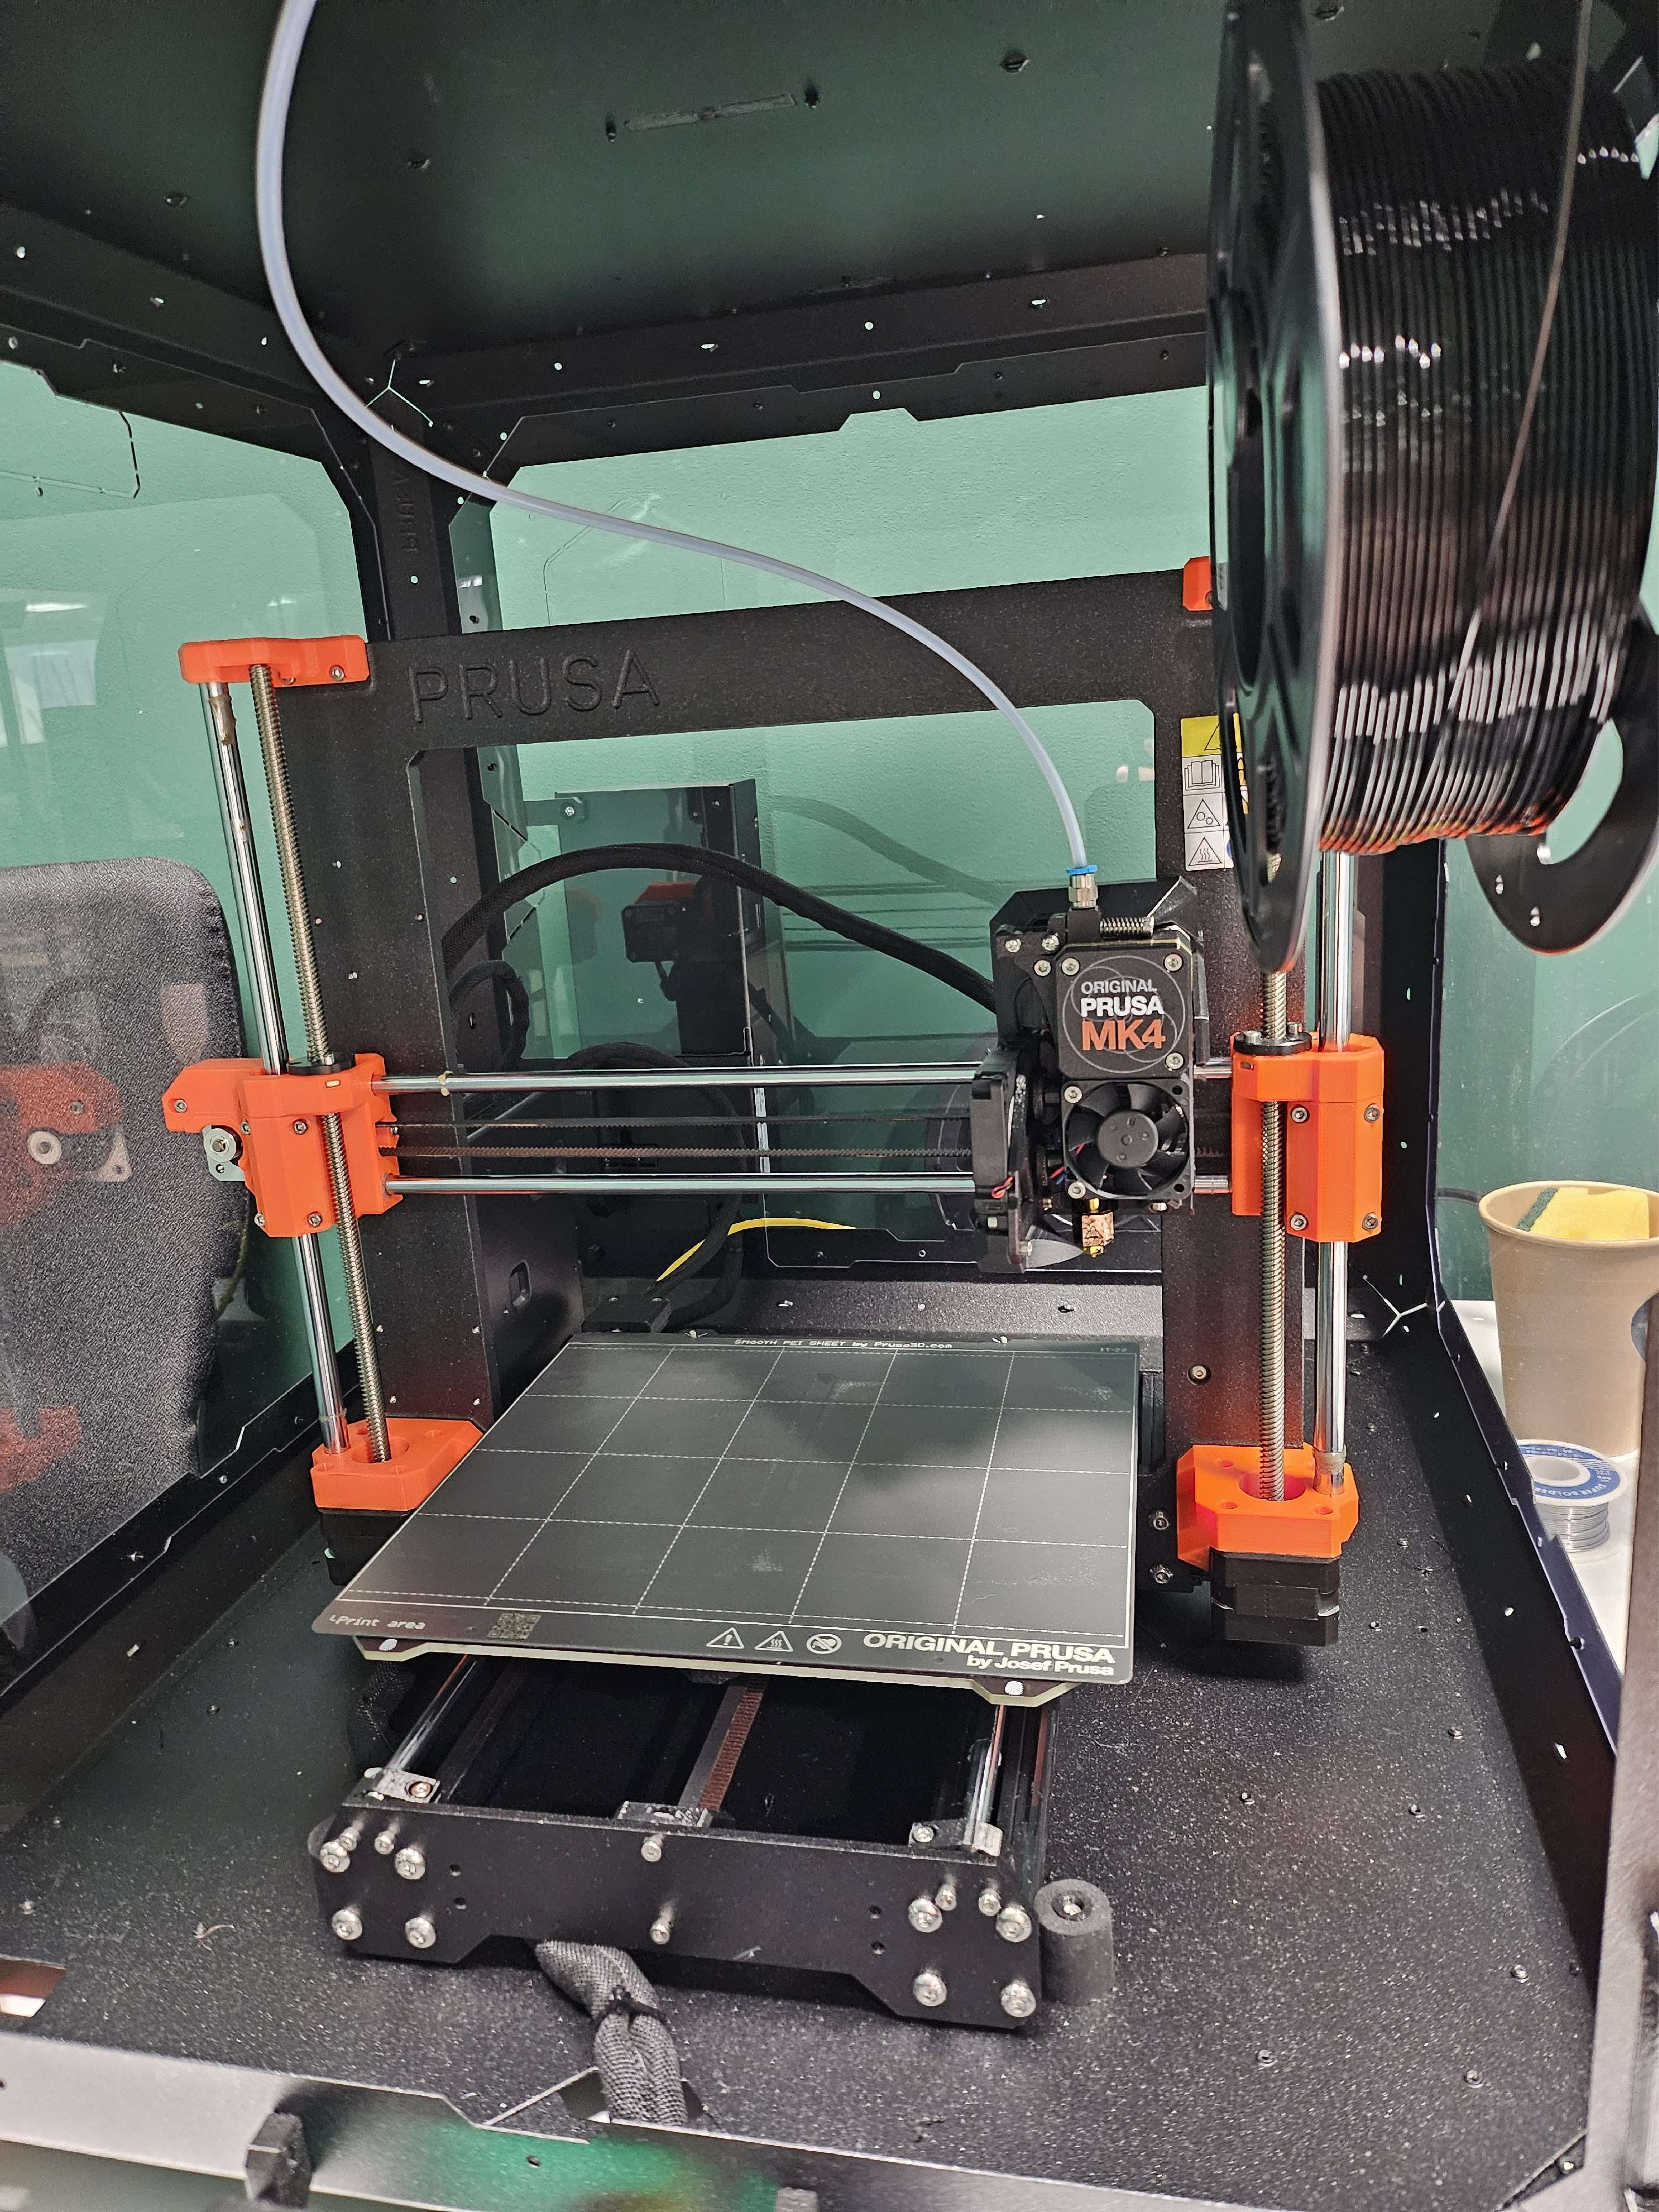
\includegraphics[width = .5\textwidth]{Imagenes/Vectorial/prusa_mk4.pdf}
	\caption{Prusa MK4 in its enclosure}
	\label{fig:prusa_mk4}
\end{figure}

\subsection{Materials}

Choosing the right material for 3D printing is critical to achieving the desired properties in the 
final product. The selection depends on various factors, including strength, flexibility, heat 
resistance, and ease of printing. Here is a brief overview of some of the most commonly used 
materials in 3D printing \cite{3dprinting_materials}:

\textbf{PLA (Polylactic Acid)}: PLA is one of the most popular materials for 3D printing due to 
its ease of use. It is made from renewable resources like corn starch and sugarcane. PLA is great 
for beginners because it prints at lower temperatures and does not require a heated bed. However, 
it is not very heat-resistant and can become brittle over time.

\textbf{ABS (Acrylonitrile Butadiene Styrene)}: ABS is a strong and durable plastic often used in 
industrial applications. It has better heat resistance compared to PLA but can be more challenging 
to print with due to its tendency to warp. ABS emits fumes during printing, so it requires a 
well-ventilated area or an enclosed printer with ventilation.

\textbf{PETG (Polyethylene Terephthalate Glycol)}: PETG is a versatile material that combines the 
ease of printing found in PLA with the strength and durability of ABS. It is also resistant to 
moisture, chemicals and UV light, making it suitable for functional parts. PETG does not warp as 
much as ABS and emits fewer fumes, making it a safer choice for indoor printing.

\textbf{Nylon}: Nylon is known for its excellent strength, flexibility, and durability. It is 
commonly used for producing parts that need to withstand mechanical stress. Nylon is more 
difficult to print with due to its tendency to absorb moisture from the air, which can affect 
print quality. Proper storage and drying are essential when using nylon.

\textbf{TPU (Thermoplastic Polyurethane)}: TPU is a flexible, rubber-like material that is ideal 
for printing items that need to be elastic and impact-resistant. It is commonly used for phone 
cases, gaskets, and wearables. TPU can be challenging to print due to its flexibility, requiring 
careful adjustments to print settings and slower print speeds.

\textbf{Composites}: Composite filaments are materials infused with fibers or powders, such as 
carbon fiber, wood, or metal. These composites can provide unique properties like increased 
strength, reduced weight, or aesthetic finishes. However, they can be abrasive and may require 
hardened steel nozzles to prevent wear during printing.

After evaluating the various materials, PETG emerged as the clear choice for the project. This 
decision was driven by several key factors. Given that some devices may be exposed to direct 
sunlight and high temperatures, PETG's excellent resistance to UV radiation and heat made it the 
most suitable material. Additionally, PETG offers a good balance of strength, flexibility, and 
ease of printing, which are crucial for creating durable and reliable enclosures. Its moisture and 
chemical resistance further enhance its suitability for this application, ensuring that the 
devices remain robust and functional in various environmental conditions.

\subsection{Printing}

With the design finalized and the material chosen, the next step is to bring the digital model to 
life through 3D printing. This section will cover the various aspects involved in the printing 
process, including printer setup, calibration and slicing the model. The aim is to ensure that the 
printed enclosures meet the required specifications and quality standards.

\subsubsection{Printer Setup and Calibration}

One of the standout aspects of the Prusa MK4 is its minimal setup and calibration requirements, 
thanks to its integrated sensors and automated processes. Upon receiving the Prusa MK4, the 
initial assembly is straightforward and well-documented, with comprehensive guides provided by 
Prusa Research. 

The Prusa MK4 is equipped with an advanced bed leveling system that uses a mesh bed leveling 
sensor. This sensor measures the distance between the print bed and the nozzle at multiple points, 
creating a precise mesh that ensures the first layer is perfectly even. This automated process 
eliminates the need for manual bed leveling, which is a common challenge with many 3D printers.

Additionally, the printer features a filament sensor that detects the presence of filament and can 
pause the print if the filament runs out or jams. This feature is particularly useful for long 
prints, ensuring that the print does not fail due to filament issues.

The Prusa MK4 includes a self-test and calibration wizard that guides users through the initial 
setup. The wizard checks all critical components, such as the print bed, extruder, and sensors, 
ensuring everything is functioning correctly before starting a print.

Due to these advanced features, the Prusa MK4 requires very little manual setup and calibration. 
Users can rely on the automated systems to handle most of the initial adjustments, allowing them 
to focus on the design and printing process rather than troubleshooting and fine-tuning the 
printer.

Furthermore, the Prusa MK4 comes with pre-configured print profiles in the \textit{PrusaSlicer} 
software. These profiles are optimized for various filament types, including PETG, and take into 
account the printer's capabilities, ensuring high-quality prints with minimal manual adjustments.

However, while the stock printing profile of the Prusa MK4 is highly optimized for general use, 
some adjustments were necessary to achieve optimal performance for the project's specific 
requirements. These modifications ensured better print quality and ease of use, particularly for 
producing PETG enclosures.

Firstly, the nozzle height was adjusted slightly by raising it 0.05mm from the bed. The default 
setting caused the nozzle to print too close to the bed, resulting in the first layer rippling due 
to excessive compression. This minor adjustment improved the first layer's smoothness and 
adhesion, providing a more consistent foundation for subsequent layers.

Additionally, the bed temperature settings were lowered. The default temperatures provided 
excellent adhesion, but this sometimes resulted in the PETG enclosure adhering too strongly to the 
print bed, making it difficult to remove without damaging the print or the bed. By reducing the 
bed temperature, sufficient adhesion was maintained for successful printing, while also allowing 
for easier removal of the completed prints.

\subsubsection{Slicing the 3D Model}

Before sending a 3D model to a 3D printer for fabrication, it must go through a crucial step known 
as slicing. Slicing is the process of converting a 3D model (typically in STL format) into a set 
of instructions (G-code) that a 3D printer can understand. This G-code provides specific 
instructions on how the printer should move its print head and build platform to create the 
desired object layer by layer.

A slicer software plays a central role in this process. It takes into account various parameters 
set by the user, such as layer height, infill density, print speed, and support structures, and 
generates the G-code accordingly. These parameters directly influence the quality, strength, and 
appearance of the final print.

Different slicer software packages are available, each with its own set of features and 
capabilities. Some popular slicers include Ultimaker Cura, PrusaSlicer, Simplify3D, and Slic3r. 
These programs offer user-friendly interfaces and a range of customization options to optimize 
prints for specific materials, print quality, and printer hardware.

For this project, PrusaSlicer was employed, as can be seen in Figures 
\ref{fig:prusaslicer_objects} and \ref{fig:prusaslicer_sliced}.

\begin{figure}[h]
    \centering
    \begin{minipage}[b]{0.47\textwidth}
        \centering
        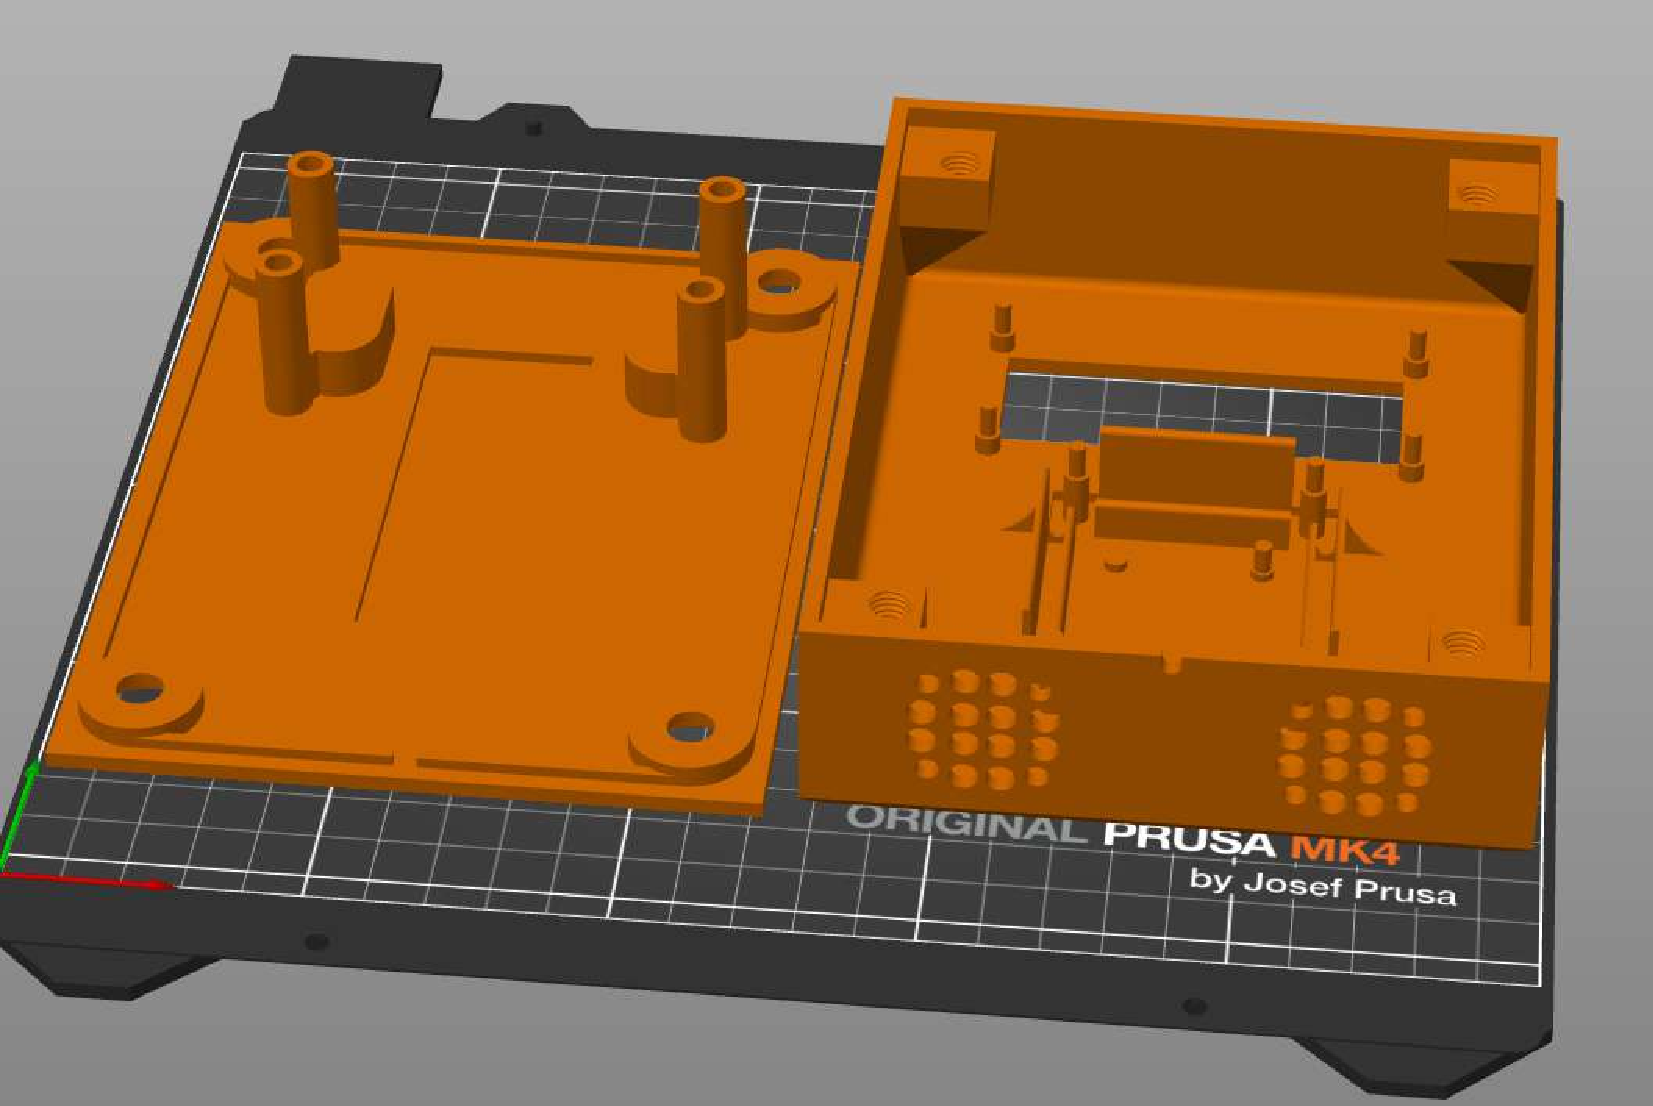
\includegraphics[width=1\textwidth]{Imagenes/Vectorial/prusaslicer_objects.pdf}
        \caption{Objects placed on the bed on PrusaSlicer}
        \label{fig:prusaslicer_objects}
    \end{minipage}
    \hfill
    \begin{minipage}[b]{0.47\textwidth}
        \centering
        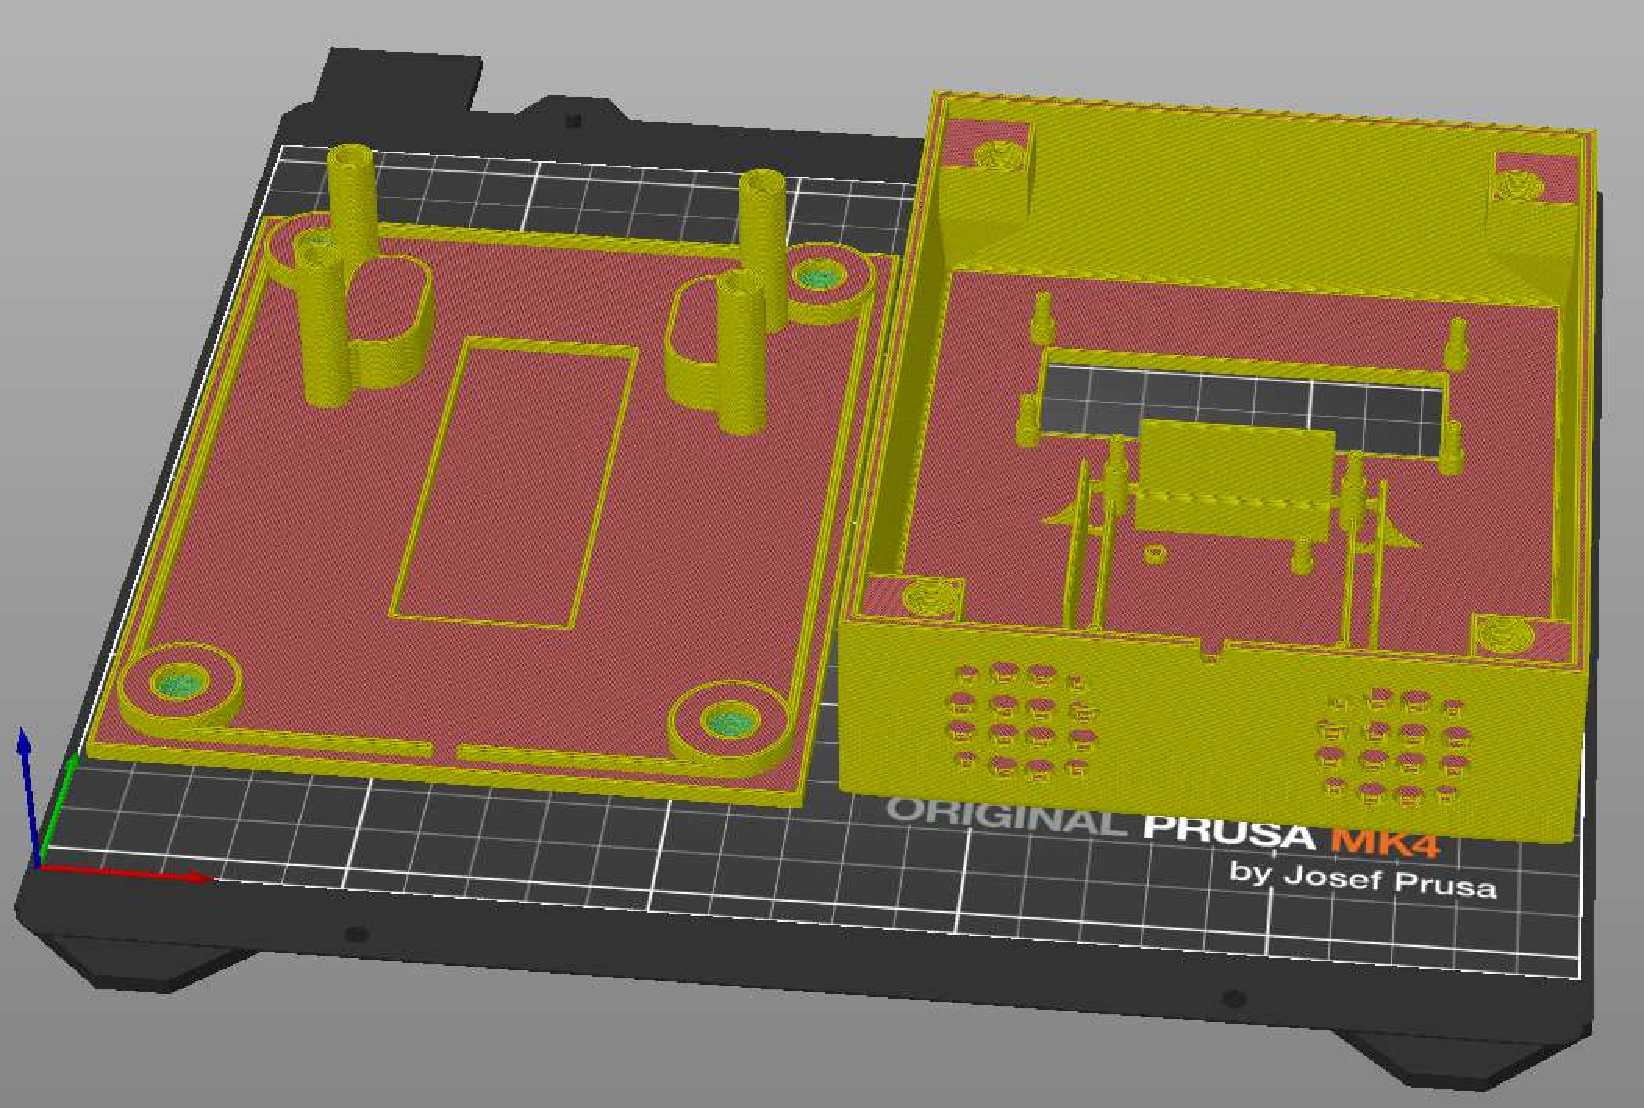
\includegraphics[width=1\textwidth]{Imagenes/Vectorial/prusaslicer_sliced.pdf}
        \caption{Sliced objects on PrusaSlicer}
        \label{fig:prusaslicer_sliced}
    \end{minipage}
\end{figure}

\subsubsection{Printing and Post-Processing}

With the 3D model sliced and the printer calibrated, the final step is straightforward: pressing 
start and waiting for the printer to finish. Once the printing process is complete, the next task 
involves removing the supports from the backplate. These supports are necessary due to the 
recesses where the screws fit, which are elevated from the print bed.

After completing this post-processing step, the printed enclosure is ready for use. The successful 
integration of the device into its newly printed enclosure can be seen in Figure 
\ref{fig:device_in_enclosure}, demonstrating the practical realization of the design and 
fabrication plan.

\begin{figure}[h]
	\centering
	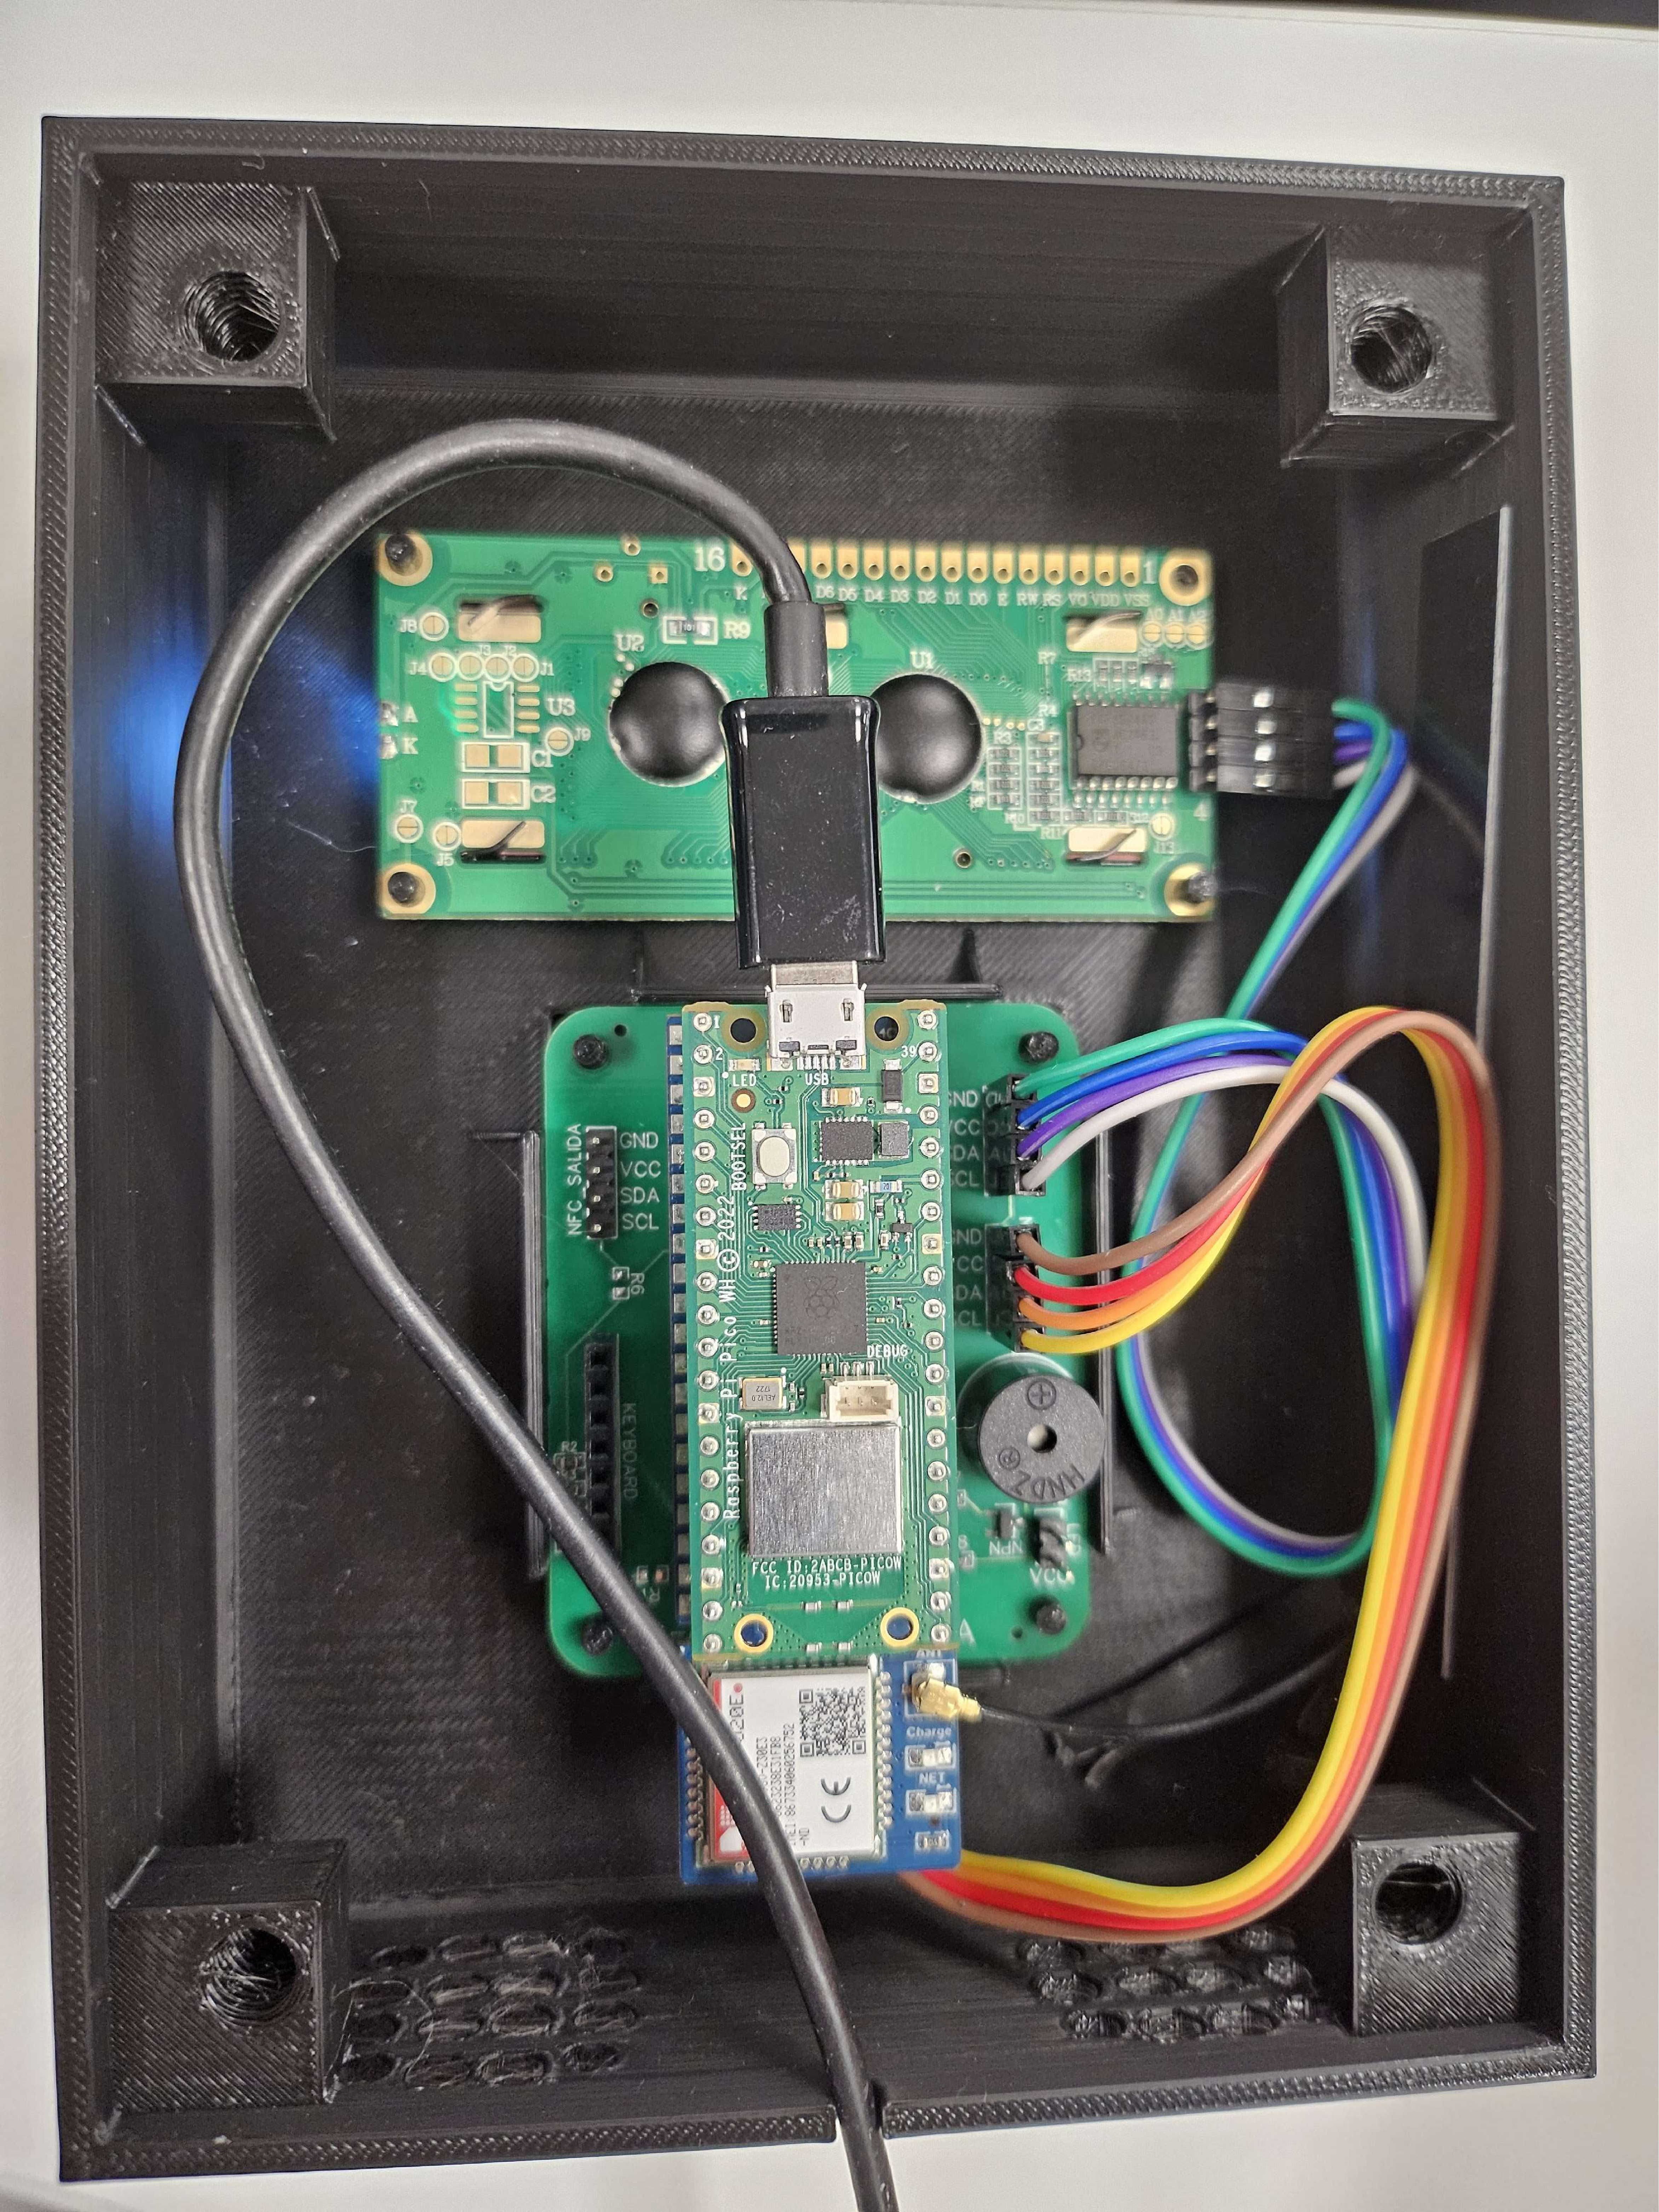
\includegraphics[width = .5\textwidth]{Imagenes/Vectorial/device_in_enclosure.pdf}
	\caption{Device in its enclosure}
	\label{fig:device_in_enclosure}
\end{figure}
